%\chapter{Common Elements in the Analysis of High Energy Physics Collision Data}
\chapter{Common Elements in the Search for New Physics}
\label{chap:common_search}

\epigraph{
\textit{Our `Age of Anxiety' is, in great part, the result of trying to do today's jobs with yesterday's tools!}
}{--Marshall McLuhan}
%Our Age of Anxiety is, in great part, the result of trying to do today’s jobs with yesterday’s tools! -- Marshall McLuhan
%Diaper spelled backwards is repaid , think about it. -- Marshall McLuhan


%%%%%%%%%%%%%%%%%%%%%%%%%%%%%%%%%%%%%%%%%%%%%%%%%%%%%%%%%%%%%%%%%%%%%%
%%%%%%%%%%%%%%%%%%%%%%%%%%%%%%%%%%%%%%%%%%%%%%%%%%%%%%%%%%%%%%%%%%%%%%

There are many ways in which physicists study and analyse the data collected by
the ATLAS detector.
Once the gathered data has been aggregated and the physics objects therein
have been reconstructed (Chapter~\ref{chap:objects}), an analysist has at their fingertips access
to the stuff of high energy particle physics from which they
can test their hypotheses or perform measurements of fundamental quantities.
In the present work, several analyses representing the search for BSM physics
will be discussed in detail.
The details of each of these analyses differ quite a bit, but each follow
a general \textit{analysis strategy} that will be discussed
further in Section~\ref{sec:gen_strategy}.
Physics analyses start with a stated goal in mind; for example,
a measurement of some quantity to a desired level of precision
or, as in the analyses to be presented, a statement about the existence of a new particle or theory of new physics.
The methods by which these statements are to be made are intertwined with, and generally
dictate the initial design of, the overall
analysis strategy and are statistical in nature.
In Section~\ref{sec:stat_hypo} a discussion of the statistical methods used
in the analyses to be presented will be given, highlighting how statements about
new physics are made and how broad-strokes physics conclusions can be drawn from them.
Section~\ref{sec:fakes} follows up on the topic of how one estimates particular sources
of SM backgrounds for which the MC simulation cannot be relied upon to give reasonable
predictions, particularly on those processes that lead to leptons being produced in the detector
that do not originate from the $pp$ hard-scatter processes of interest.

%%%%%%%%%%%%%%%%%%%%%%%%%%%%%%%%%%%%%%%%%%%%%%%%%%%%%%%%%%%%%%%%%%%%%%
%%%%%%%%%%%%%%%%%%%%%%%%%%%%%%%%%%%%%%%%%%%%%%%%%%%%%%%%%%%%%%%%%%%%%%
%
% GENERAL STRATEGY
%
%%%%%%%%%%%%%%%%%%%%%%%%%%%%%%%%%%%%%%%%%%%%%%%%%%%%%%%%%%%%%%%%%%%%%%
%%%%%%%%%%%%%%%%%%%%%%%%%%%%%%%%%%%%%%%%%%%%%%%%%%%%%%%%%%%%%%%%%%%%%%
\section{General Analysis Strategy}
\label{sec:gen_strategy}

In this section the analysis strategy used in the searches for new physics
to be presented in Chapters~\ref{chap:search_stop2l} and \ref{chap:search_bbww}
will be given.
The general analysis workflow for designing an analysis is outlined in the following
sub-sections.

%%%%%%%%%%%%%%%%%%%%%%%%%%%%%%%%%%%%%%%%%%%%%%%%%%%%%%%%%%%%%%%%%%%%%%%%%%%%%
% SIGNAL PHENO
%%%%%%%%%%%%%%%%%%%%%%%%%%%%%%%%%%%%%%%%%%%%%%%%%%%%%%%%%%%%%%%%%%%%%%%%%%%%%
\subsection{Target the Signal}
\label{sec:sig_pheno}

The search for a particular source of new physics, such as a particular model of SUSY (Chapter~\ref{chap:bsm}),
begins first with the thorough understanding of the signatures that the new physics model
will leave in the ATLAS detector.
This generally requires a strict definition of the \textit{final state} of the
new physics model that one wishes to look for; for example, deciding to search for
evidence of SUSY via the production of the SUSY partners to the SM top-quark
in final states having exactly two leptons (electrons or muons) instead of
exactly zero or exactly one lepton, as in Chapter~\ref{chap:search_stop2l}.\footnote{Performing
searches for new physics by the partitioning of specific new physics models
by their resulting final states allows for separate, independent dedicated analyses to be carried out
for each possible final state with the idea that each one will be more sensitive
to the presence of the new physics in their respective final state than would be
a single analysis attempting to target all possible final states of the new physics production.
The results of the independent analyses' searches can be statistically combined once they are finished,
leading to enhanced sensitivities to the new physics scenario in question that is more or less independent
of the final state.}
Once a new physics model has been chosen, along with its final state, there is a well-defined
\textit{signal} to be looked for in the data recorded by the ATLAS detector.
The production and decay of the sought-for signal is then simulated via MC methods in the exact
same manner as for the SM processes, as described in Chapter~\ref{chap:simulation}.
In physics analyses, the physics processes not inclusive of the sought-for signal processes
are referred to as the \textit{background} processes.

The simulation of the signal process allows one to study the kinematics of the signal in detail, in order
to get an overall feel for what phase space the signal inhabits.
Knowledge of both the signal final state and its kinematics therein informs the analyst
about the specific SM background processes that are likely to be relevant to the analysis.
For example, if the sought-for signal decays to two leptons with opposite electric charge
that are of the same flavor (both leptons are electrons or both are muons, for example)
it is very likely that the SM processes inclusive of $Z$-boson production will be relevant,
since this is one of the main $Z$-boson decay final states, as opposed to the production of a single $W$-boson
whose decay does not lead directly to final states with two leptons.
Knowledge of the dominant SM background processes, then, allows
one to determine how the phenomenology and kinematics of the signal differ
with respect to those of the relevant backgrounds by comparing the simulated events
of each.
The aim of this is to be able to define a basis of kinematic observables that allows
for the discrimination between the signal and background.
From such a basis of observables, one can define regions of phase space in which
the signal-to-background ratio is large, such that the likelihood of observing
the presence of the signal is (ideally) maximal.
Such regions of increased signal purity\footnote{The `purity' of a process is defined
as the fraction of a given process in a region of phase space, relative to the sum
of all processes (inclusive of the process in question).} are referred
to as \textit{signal regions} (SR).
As an example, take the case where there is a single discriminating variable in our
basis of useful kinematic observables.
One would apply a selection on this observable in such a way that $pp$ collision events
satisfying this selection are likely to be enhanced in signal events.
This is one-diminsional SR case is illustrated in Figure~\ref{fig:sr_search_v}.

\begin{figure}[!htb]
    \begin{center}
        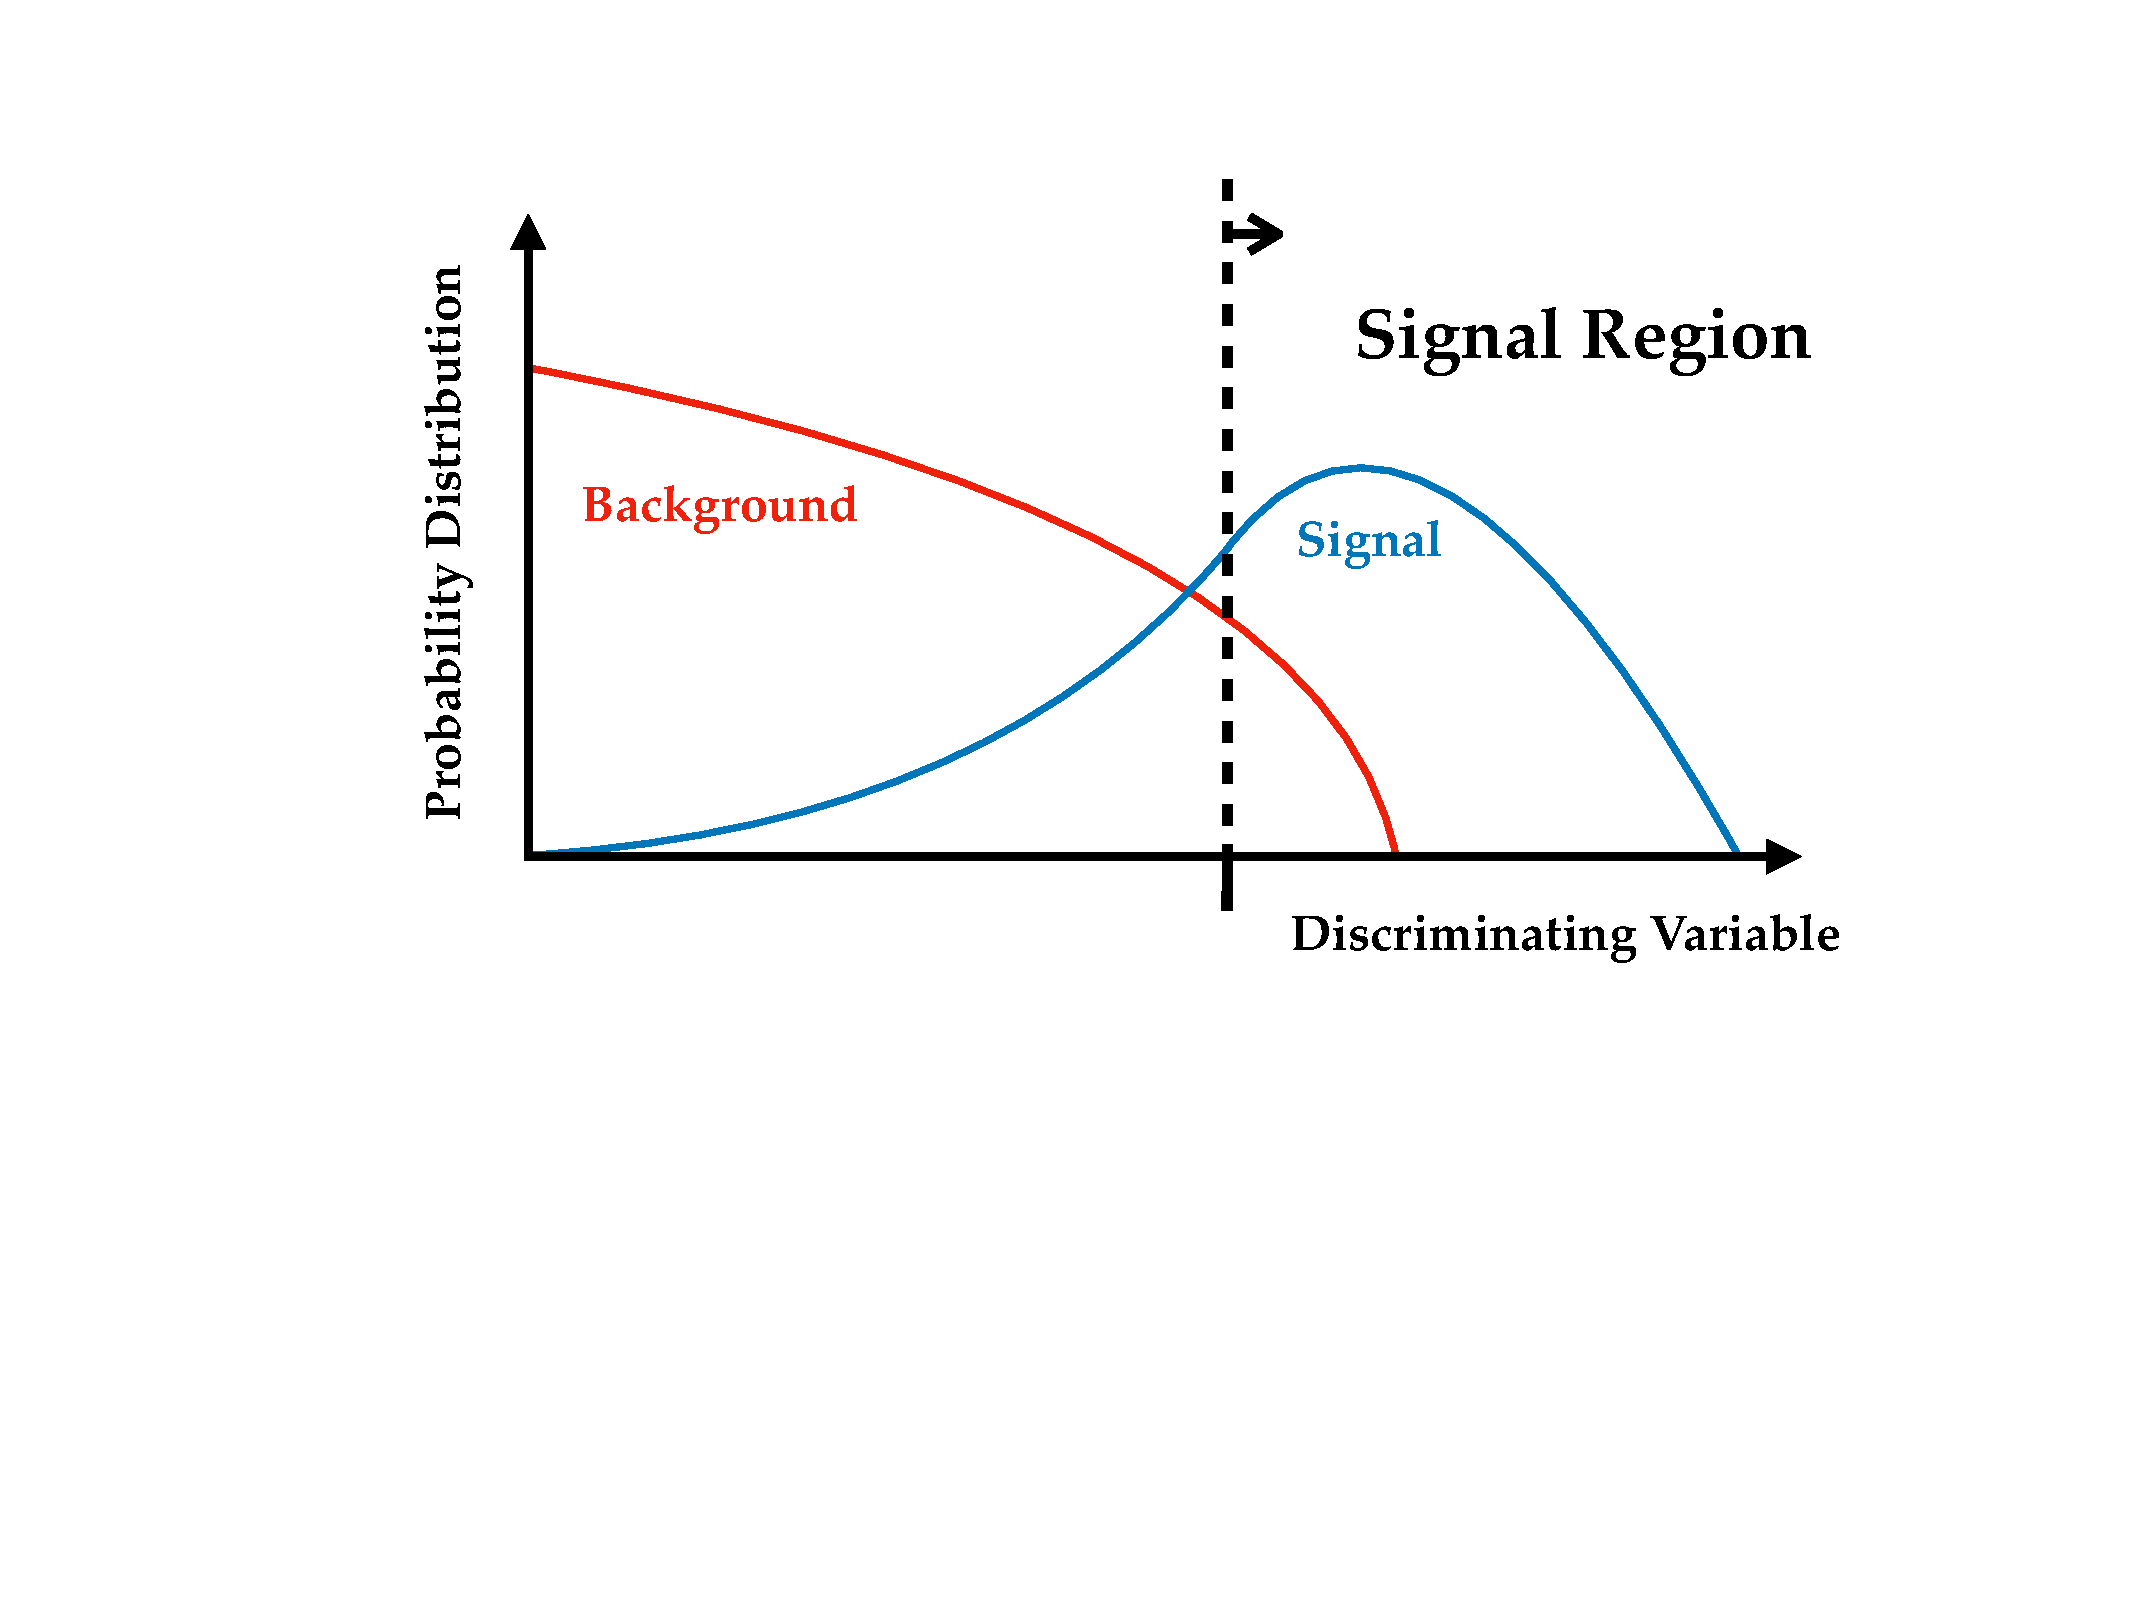
\includegraphics[width=0.65\textwidth]{figures/common_ana/sr_search_vPDF}
        \caption{
            Signal region concept illustrated in the case of a one-dimensional selection
            made on a discriminating kinematic observable.
            The dominant SM background (red) is characterised by typically small values
            of the discriminating variable whereas the signal (blue) has values that extend
            beyond that of the background.
            The signal region in this case is defined by requiring $pp$ collision events
            to have values of the discriminating variable that are larger than
            the value indicated by the dashed vertical line, where the signal purity is
            enhanced.
        }
        \label{fig:sr_search_v}
    \end{center}
\end{figure}



%%%%%%%%%%%%%%%%%%%%%%%%%%%%%%%%%%%%%%%%%%%%%%%%%%%%%%%%%%%%%%%%%%%%%%%%%%%%%
% GATHER THE DATA
%%%%%%%%%%%%%%%%%%%%%%%%%%%%%%%%%%%%%%%%%%%%%%%%%%%%%%%%%%%%%%%%%%%%%%%%%%%%%
\FloatBarrier

%%%%%%%%%%%%%%%%%%%%%%%%%%%%%%%%%%%%%%%%%%%%%%%%%%%%%%%%%%%%%%%%%%%%%%%%%%%%%
% THE CONTROL REGION METHOD
%%%%%%%%%%%%%%%%%%%%%%%%%%%%%%%%%%%%%%%%%%%%%%%%%%%%%%%%%%%%%%%%%%%%%%%%%%%%%
\subsection{Background Estimation and the Control Region Method}
\label{sec:control_region_method}

The general principle behind searches for new physics is to define a SR, or a set of SRs,
and then make predictions about how the signal and background behave therein.
Such predictions can then be compared to the data actually recorded by the ATLAS detector
and the statistical procedures described in Section~\ref{sec:stat_hypo} can be used to
make statements about whether or not --- or to what degree --- the data is likely to contain the specified signal.
The emphasis, then, in physics analyses is on the understanding and precise estimation of the backgrounds.
Without being able to properly estimate the contribution of the background processes to the
events in the SRs well-defined predictions cannot therein be made, resulting in ineffective
analyses.

The process of estimating the backgrounds in an analysis' SRs is aptly referred to as
\textit{background estimation}.
There are many background estimation methods that are used.
There exist general background estimation techniques, applicable to a wide range of SM processes,
as well as more dedicated estimation techniques that are specific to a smaller subset of
SM processes.
Most rely on the MC simulation of the SM processes, either as the primary source of providing
the prediction of a given SM process in an analysis' SR(s) or secondarily, as a means of providing a
cross-check on a prediction obtained using data.
The high levels of accuracy imposed upon the ATLAS MC simulation infrastructure is derived
from the large and dominant role that the MC simulation plays in the background estimation
procedures in almost all analyses performed by the ATLAS experiment.

\begin{figure}[!htb]
    \begin{center}
        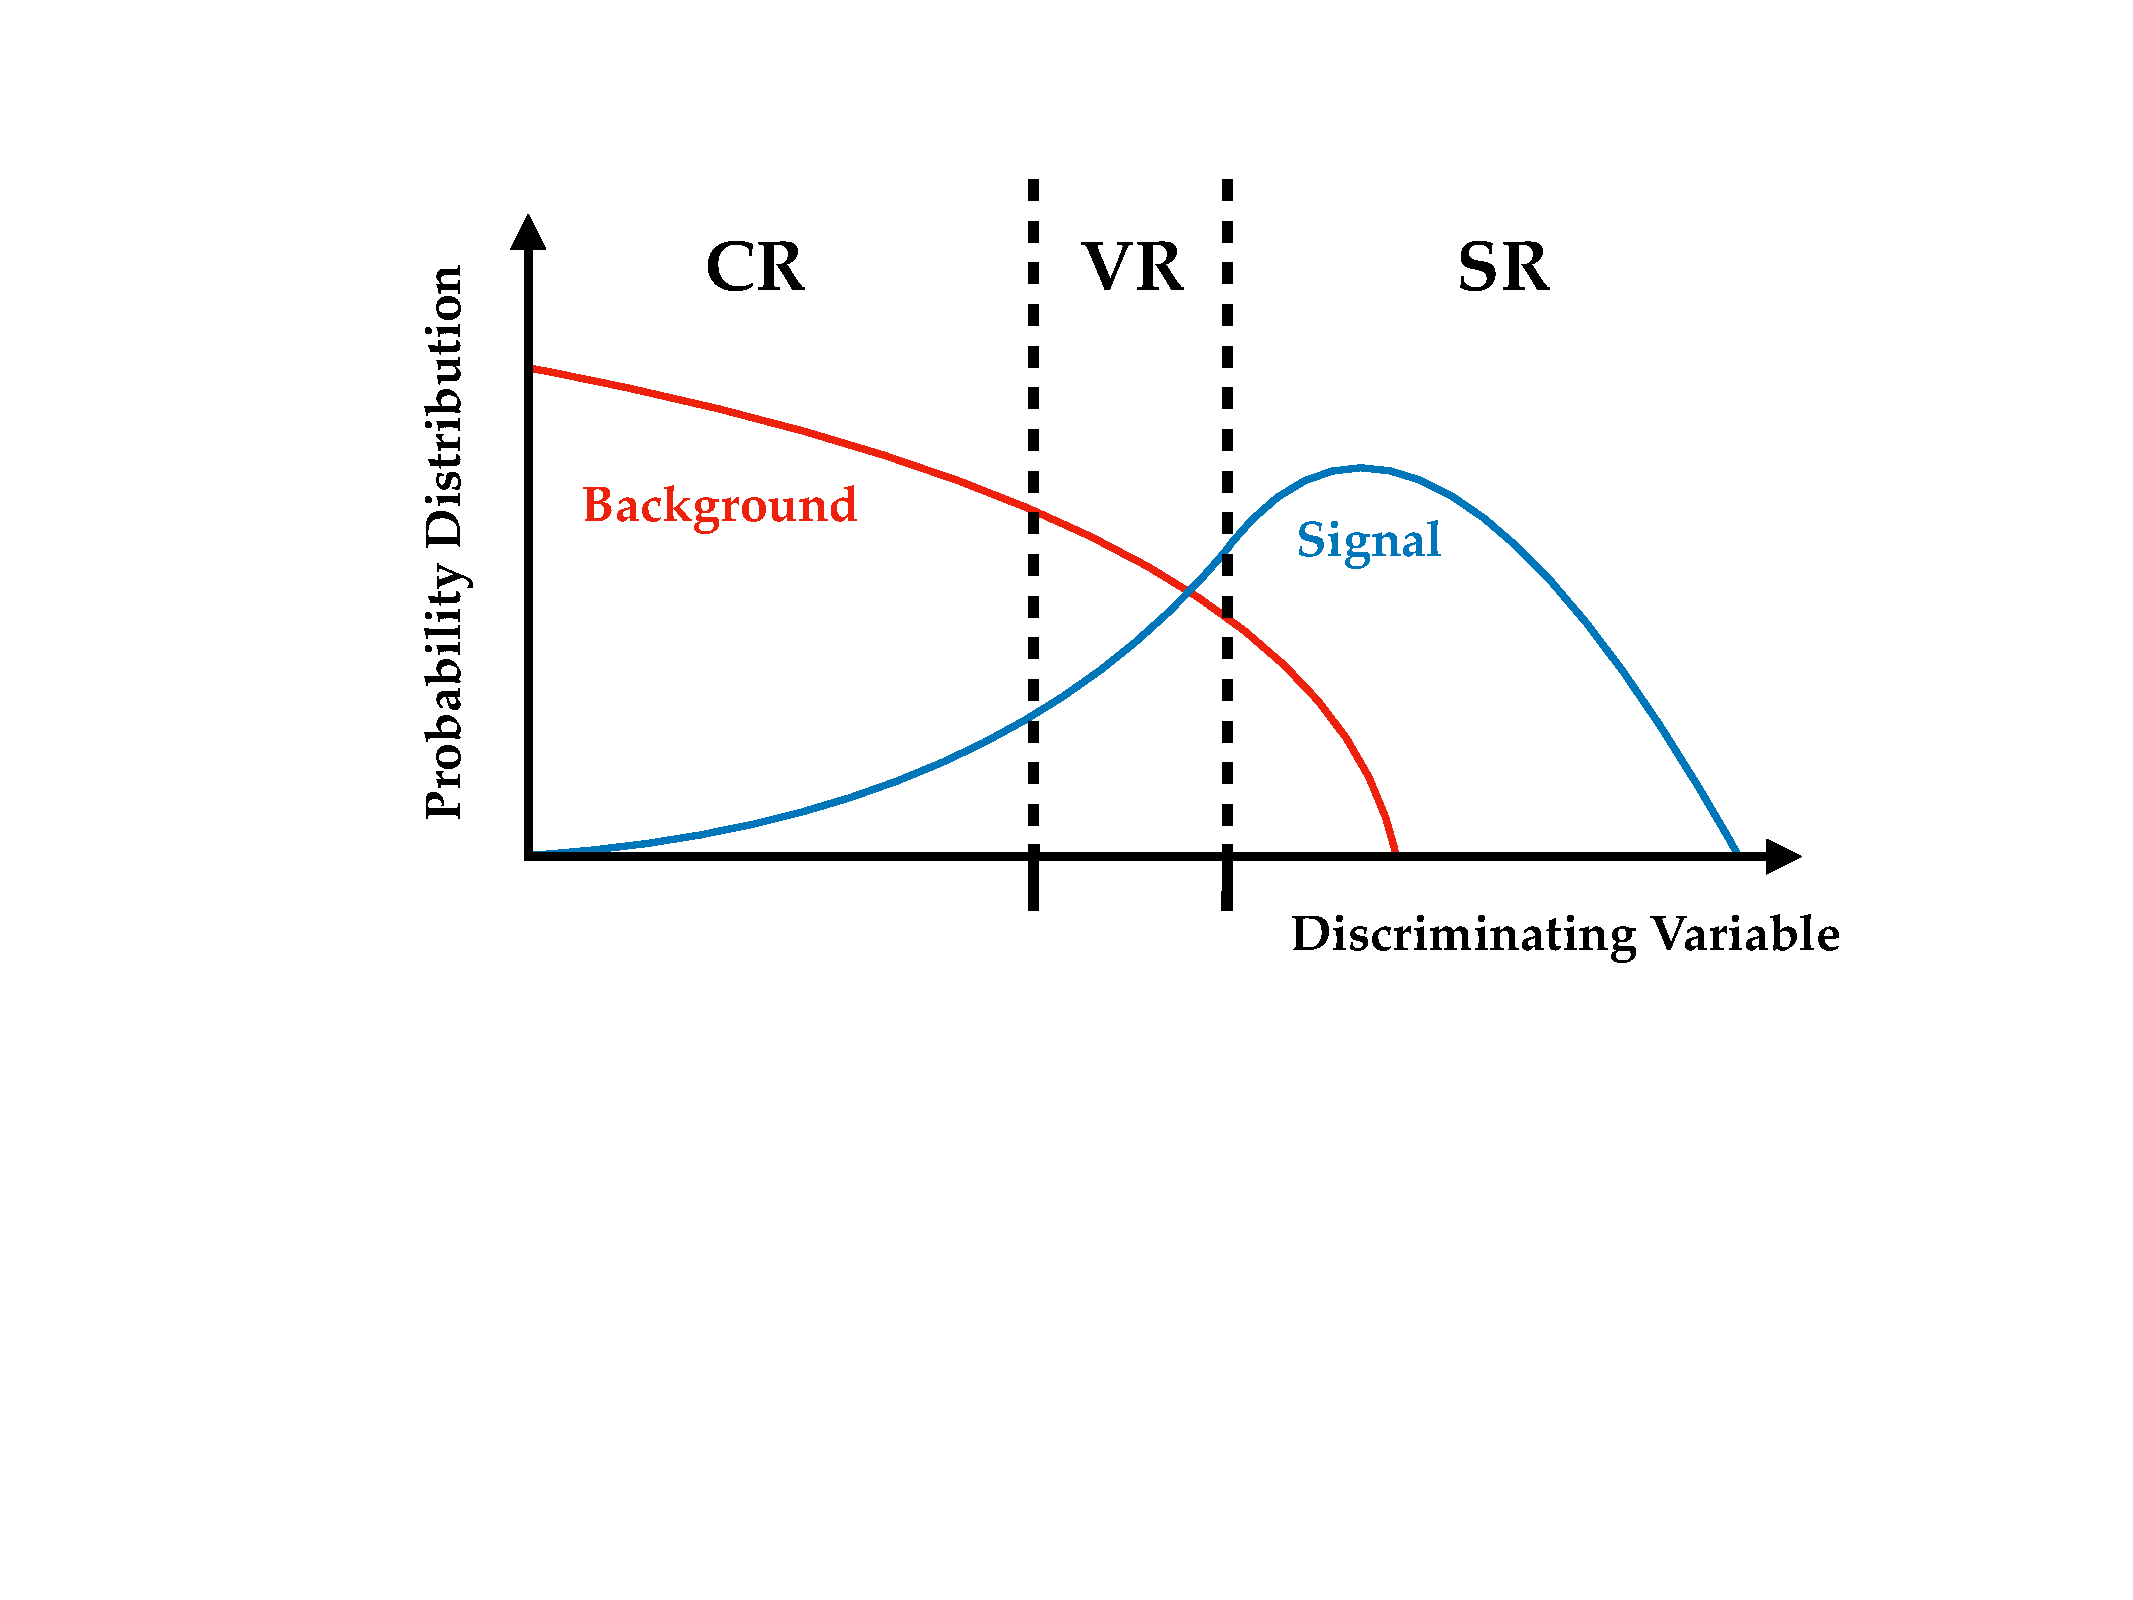
\includegraphics[width=0.65\textwidth]{figures/common_ana/sr_search_v_CRPDF}
        \caption{
        }
        \label{fig:sr_search_v_CR}
    \end{center}
\end{figure}

%%%%%%%%%%%%%%%%%%%%%%%%%%%%%%%%%%%%%%%%%%%%%%%%%%%%%%%%%%%%%%%%%%%%%%%%%%%%%
% SYSTEMATIC UNCERTAINTIES
%%%%%%%%%%%%%%%%%%%%%%%%%%%%%%%%%%%%%%%%%%%%%%%%%%%%%%%%%%%%%%%%%%%%%%%%%%%%%


%%%%%%%%%%%%%%%%%%%%%%%%%%%%%%%%%%%%%%%%%%%%%%%%%%%%%%%%%%%%%%%%%%%%%%
%%%%%%%%%%%%%%%%%%%%%%%%%%%%%%%%%%%%%%%%%%%%%%%%%%%%%%%%%%%%%%%%%%%%%%
%
% STATISTICS AND HYPOTHESIS TESTING
%
%%%%%%%%%%%%%%%%%%%%%%%%%%%%%%%%%%%%%%%%%%%%%%%%%%%%%%%%%%%%%%%%%%%%%%
%%%%%%%%%%%%%%%%%%%%%%%%%%%%%%%%%%%%%%%%%%%%%%%%%%%%%%%%%%%%%%%%%%%%%%
\section{Hypothesis Testing and Statistics}
\label{sec:stat_hypo}

This section describes the statistical procedures used in the analyses to be
presented in Chapters~\ref{chap:seach_stop} and \ref{chap:search_hh} that allow
for conclusions to be drawn about the compatibility of the observed data with theories of
BSM physics.
The statistical inference tools described are inherently Frequentist and
are, for the most part, the \textit{de facto} standard for physics analyses searching for evidence of BSM physics
at the large experiments at the LHC.
Their widespread adoption by the experiments at the LHC does not indicate the
philosophical merit of Frequentist inference methodology, but rather highlights the technically simple implementation
of Frequentist hypothesis testing that allows for physics analyses to not get
bogged down in some of the details associated with Bayesian analyses, computational
or otherwise.
Indeed, most people by default think and interact with the world around them
in a Bayesian manner.
Taking the path of least resistance, physicists have tended to opt for the simpler
implementation of reporting their results, which, at the end of the day,
tend to not lose out much in terms of the picture of the objective truth that they draw~\cite{CousinsBayes}.
Section~\ref{sec:hypo_test} will describe, in somewhat general terms, what
hypotheses tests are and the way in which they are performed in ATLAS.
Section~\ref{sec:likelihood} describes the details by which the measurements and systematic
uncertainties of
an analysis are transcribed into the language of the hypothesis test described
in Section~\ref{sec:hypotest} using a likelihood-based test statistic.


%%%%%%%%%%%%%%%%%%%%%%%%%%%%%%%%%%%%%%%%%%%%%%%%%%%%%%%%%%%%%%%%%%%
%%%%%%%%%%%%%%%%%%%%%%%%%%%%%%%%%%%%%%%%%%%%%%%%%%%%%%%%%%%%%%%%%%%
%
% HYPOTHESIS TESTING
%
%%%%%%%%%%%%%%%%%%%%%%%%%%%%%%%%%%%%%%%%%%%%%%%%%%%%%%%%%%%%%%%%%%%
%%%%%%%%%%%%%%%%%%%%%%%%%%%%%%%%%%%%%%%%%%%%%%%%%%%%%%%%%%%%%%%%%%%

\subsection{Hypothesis Testing and the \cls Construction}
\label{sec:hypo_test}

Hypothesis testing starts with the unambiguous formulation of the hypothesis being
tested.
In the search for evidence of BSM physics, there are two hypothesis pitted
against one another.
The first is the \textit{null hypothesis}, denoted $H_0$, which is the hypothesis
subject to the test and corresponds to the SM hypothesis. The null hypothesis is commonly
referred to simply as the background-only (B) hypothesis.
The second hypothesis is the \textit{alternate hypothesis}, denoted $H_1$, and corresponds
to the SM with the addition of the BSM physics process being sought out.
The hypothesis $H_1$ is commonly referred to as the signal-plus-background (S+B) hypothesis.
In both searches presented in Chapters~\ref{chap:search_stop} and \ref{chap:search_hh},
$H_0$ is taken to be the SM.
In the search presented in Chapter~\ref{chap:search_stop}, $H_1$ is taken to be a specific
instantiation of the MSSM ({\color{red}{Section XXX}}), with specific masses of the
stop quark and LSP.
In the search presented in Chapter~\ref{chap:search_hh}, $H_1$ is taken to be the
non-resonant production of Higgs boson pairs.
In this latter case, the $H_1$ hypothesis is indeed a process predicted by the SM ({\color{red}{SECTION XXX about HH pheno and EWSB}}) but
it is one that is not included in the $H_0$ hypothesis.

%%%%%%%%%%%%%%%%%%%%%%%%%%%%%%%%%%%%%%%%%%%%%%%%%%%%%%%%%%%%%%%%%%%
%%%%%%%%%%%%%%%%%%%%%%%%%%%%%%%%%%%%%%%%%%%%%%%%%%%%%%%%%%%%%%%%%%%
%
% TEST STATISTICS
%
%%%%%%%%%%%%%%%%%%%%%%%%%%%%%%%%%%%%%%%%%%%%%%%%%%%%%%%%%%%%%%%%%%%
%%%%%%%%%%%%%%%%%%%%%%%%%%%%%%%%%%%%%%%%%%%%%%%%%%%%%%%%%%%%%%%%%%%
\subsubsection{The Test Statistic and $p$-Values}

In order to perform a hypothesis test in the Frequentist arena, a \textit{test statistic}, $q(x)$,
is defined.
A test statistic is defined using the analysis' measurements $x$ alone and is
used in order to define metrics by which the observed data is said to agree with
one of the two hypothesis, either $H_0$ or $H_1$.
In Section~\ref{sec:likelihood}, the exact form of the likelihood used in modern LHC experiments,
and that used in the analyses discussed in Chapters~\ref{chap:search_stop} and \ref{chap:search_hh},
will be introduced.
Here we will discuss general features of Frequentist test statistics and introduce
some of the language that will be used later on when discussing the results of the
analyses.

The conclusions eventually drawn about a given hypothesis are based on the observed value
of $q(x)$ and where this value lies in relation to the pre-defined \textit{critical region}.
The critical region is defined by a cut value, $q_c$, on the distribution of $q(x)$ under a specified hypothesis.
In the one-sided tests to be considered in the present thesis, $H_1$
will tend to have larger values of $q(x)$ as compared to $H_0$.
The critical region defines two important parameters associated with the hypothesis test.
The first is the quantity $\alpha$, which is referred to as the \textit{significance level},
and is defined as follows,
\begin{align}
    \int\limits_{q_c}^{+\infty} \, f(q | H_0) \, \mathrm{d}q = \alpha,
    \label{eq:sig_level}
\end{align}
where $f(q|H_0)$ is the probability distribution for the test statistic under
the background-only hypothesis.
The quantity $\alpha$ reports the probability for the background-only hypothesis (the SM) to be rejected when it is actually
true. This is commonly referred to as the Type I error rate.
The second quantity is $\beta$ and is defined as,
\begin{align}
    \int\limits_{-\infty}^{q_c} \, f(q|H_1) \, \mathrm{d}q = \beta,
    \label{eq:power_level}
\end{align}
where $f(q|H_1)$ is the probability distribution for the test statistic under
the signal-plus-background hypothesis.
The quantity $\beta$ gives the probability to reject the signal-plus-background hypothesis
when it is actually true. This is commonly referred to as the Type II error rate.
The quantity $(1-\beta)$ is referred to as the \textit{power of the test}.
The better a given physics analysis is at being able to discriminate between the signal
and background, i.e. to have clear separation between the $H_0$ and $H_1$ hypotheses,
the smaller (larger) is $\beta$ (the power of the test).

For simplicity, the two hypotheses $H_0$ and $H_1$ can be generalised by introducing a so-called
`signal strength' parameter, $\mu$, which acts as a multiplicative factor on the signal cross-section
appearing in $H_1$.
The hypothesis $H_0$, then, corresponds to the case $\mu = 0$ and that of $H_1$ corresponds to
$\mu = 1$.
With this general notation, then, the test statistic under either hypothesis is labelled as $q_{\mu}$.

Once a test statistic is specified, and its expected distribution under a given hypothesis is obtained,
$p$-values can be defined in order to compute the probability that the observed data originates from the
considered hypothesis (value of $\mu$).
They are computed as follows,
\begin{align}
    p_{\mu} = \int\limits_{q_{\mu, \text{obs}}}^{+\infty} \, f(q_{\mu} | \mu) \, \mathrm{d}q_{\mu},
    \label{eq:test_stat_pvalue}
\end{align}
where $q_{\mu, \text{obs}}$ is the observed value of the test statistic in data and $f(q_{\mu} | \mu)$ is the probability
density function of $q_{\mu}$ assuming hypothesis $\mu$.
A particular case of Equation~\ref{eq:test_stat_pvalue} is that of $p_0$, which quantifies the agreement of the data with the background-only
hypothesis ($\mu = 0$).
The $p_{\mu}$-value associated with a given hypothesis ($\mu$-value) is typically converted into the equivalent corresponding Gaussian significance, $Z$, defined
as the number of standard deviations that correspond to an upper-tail probability of $p_{\mu}$.
This is illustrated in Figure~\ref{fig:pval_sig}.

As the value of $p_{\mu}$ gets smaller, the confidence that the assumed hypothesis (value of $\mu$) is true
decreases.
At a certain point, it becomes acceptable to say that the assumed hypothesis is incompatible with
reality and the hypothesis described by the particular value of $\mu$ is said to be \textit{excluded}.
In the particle physics community, the conventional threshold to take for the value of $p_{\mu}$
at which point a hypothesis is said to be excluded is $p_{\mu} = 0.05$, corresponding to $Z=1.64$ as
illustrated in Figure~\ref{fig:pval_sig}.
This choice of the $p_{\mu}$-value at which point exclusion is said to occur defines
the critical region, described above, of the test.
The value of $0.05$ corresponds to the significance level of the test (c.f. Equation~\ref{eq:sig_level}), and is referred
to a hypothesis test being performed at the $95\%$ confidence level (CL) (i.e. CL $\equiv (1-\alpha)$)

In order to claim that new physics has been seen, the null hypothesis ($\mu = 0$) must be rejected.
The thresholds at which new physics can be said to have been observed and discovered are
much more stringent than that used for the exclusion of a specified hypothesis.
Incompatibilities with the null-hypothesis at the level of $p_0 = 1.3 \times 10^{-3}$ and
$p_0 = 2.9\times 10^{-7}$ are required in order to state that observation and discovery, respectively,
of new phenomena has occurred.
These thresholds, illustrated in Figure~\ref{fig:pval_sig}, for claiming observation and discovery are the fabled `$3\sigma$' and `$5\sigma$'
$p_0$-value criterion adopted by the particle physics community.

\begin{figure}[!htb]
    \begin{center}
        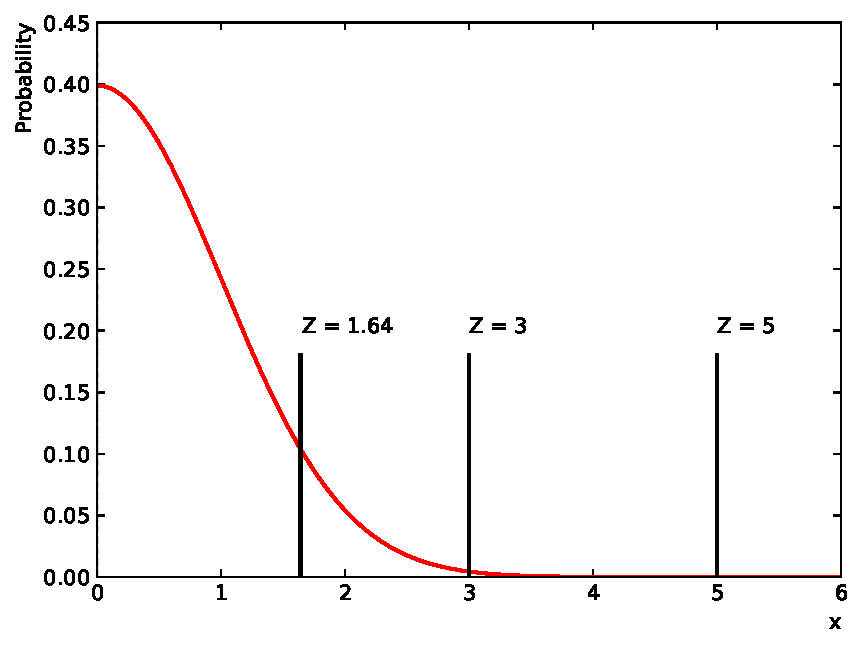
\includegraphics[width=0.48\textwidth]{figures/common_ana/stat_hypo/pval_sig_lin}
        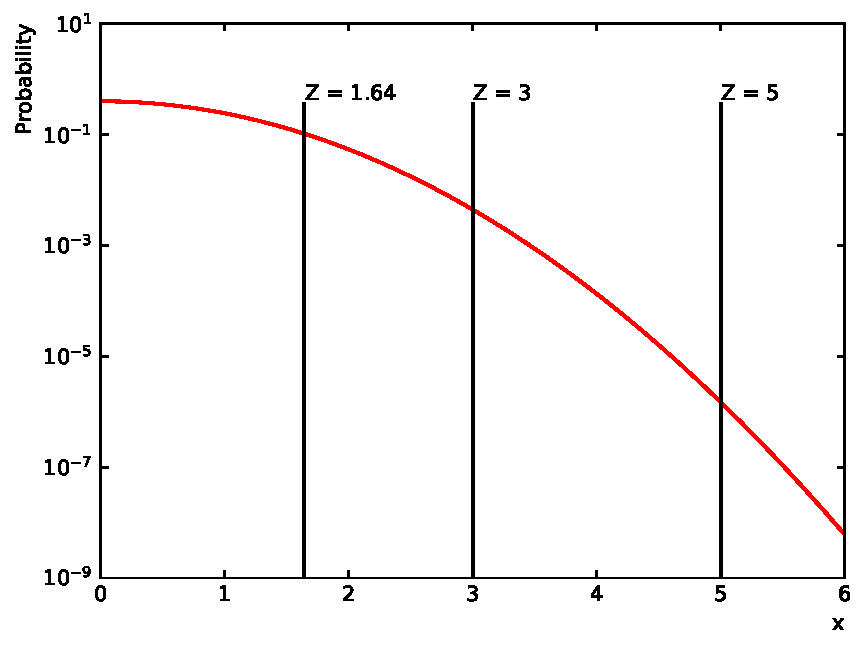
\includegraphics[width=0.48\textwidth]{figures/common_ana/stat_hypo/pval_sig_log}
        \caption{
            Gaussian tail significance levels corresponding to specific $p$-values.
            The significance level of $Z=1.64\sigma$ corresponds to $p = 0.05$,
            that of $Z=3\sigma$ to $p = 1.3 \times 10^{-3}$, and that of
            $Z = 5\sigma$ to $p = 2.9\times 10^{-7}$.
            The area under the tail to the right of each indicated significance level corresponds to
            the associated $p$-value.
            \textbf{\textit{Left}}: Linear $y$-scale. \textbf{\textit{Right}}: Logarithmic $y$-scale.
        }
        \label{fig:pval_sig}
    \end{center}
\end{figure}

%The process of performing a hypothesis test, then, is specified by the following procedure:
%\begin{enumerate}
%    \item Unambiguously define the background-only (the SM prediction) and signal-plus-background (the prediction of the SM with BSM physics added)
%            hypotheses, $H_0$ and $H_1$.
%    \item Define an appropriate test statistic, $t(x)$ (see Section~\ref{sec:likelihood}).
%    \item Construct the distribution of the test statistic under the background-only hypothesis, $g(t|H_0)$.
%    \item Define the desired significance level of the hypothesis, $\alpha$
%    \item Obtain the value of $t(x)$ as observed in data
%    \item If the observed value of $t(x)$ is within the critical region defined by $\alpha$ as in Equation~\ref{eq:sig_level} ($t_{\text{obs}} > t_c$), reject $H_0$.
%            Otherwise, $H_0$ cannot be rejected.
%\end{enumerate}


%%%%%%%%%%%%%%%%%%%%%%%%%%%%%%%%%%%%%%%%%%%%%%%%%%%%%%%%%%%%%%%%%%%
%%%%%%%%%%%%%%%%%%%%%%%%%%%%%%%%%%%%%%%%%%%%%%%%%%%%%%%%%%%%%%%%%%%
%
% THE CLS METHOD
%
%%%%%%%%%%%%%%%%%%%%%%%%%%%%%%%%%%%%%%%%%%%%%%%%%%%%%%%%%%%%%%%%%%%
%%%%%%%%%%%%%%%%%%%%%%%%%%%%%%%%%%%%%%%%%%%%%%%%%%%%%%%%%%%%%%%%%%%

\subsubsection{The \cls Construction}
\label{sec:cls_method}

In searches for new physics, the statement that a given signal hypothesis has been excluded
is an important one.
Once made by the LHC experiments, the specific signal model is essentially considered
no longer important to be searched for.
Therefore, the metrics by which the experiments make claims of exclusion have surrounding them
a wide-ranging literature discussing the merits and drawbacks of the many such metrics
that have been proposed over the years.
The bare $p_{\mu}$-value, for example, extracted from the observed data is subject to statistical fluctuations
and it can lead to unphysical exclusions when a downward fluctuation in the observed
number of events occurs.
This would lead to a premature exclusion of perhaps a broad region of new physics
that would perhaps no longer be looked into by future analyses or experiments.

The standard metric used by the LHC experiments today is known as `\cls'~\cite{CLSReadI,CLSReadII},
and is constructed in such a way as to reduce the likelihood of excluding signal
hypotheses that a search is not a-priori sensitive to.
The \cls metric is given by,
\begin{align}
    \text{CL}_s = \frac{p_{\mu}}{1-p_0},
    \label{eq:cls_def}
\end{align}
where the quantities $p_{\mu}$ and $p_0$ quantify the compatibilities between the data and the signal-plus-background
and background-only hypotheses, respectively.
Downward fluctuations in data, as those described above, will lead to larger values of $p_0$; thus
leading to larger values of \cls that avoid premature exclusion.

At the LHC, the \cls metric is used primarily for performing hypothesis tests aimed at claiming exclusion.
The standard null-hypothesis $p_0$-value is still used for claiming observation and discovery, as described above.
A given signal hypothesis with $\mu = 1$ is considered excluded when $\cls \le 0.05$.
Note that this prescription for exclusion, $\cls \le \alpha$, is generally a stronger requirement than the
standard prescription, $p_{\mu} \le \alpha$.
The \cls metric is also used to compute \textit{upper limits}.
An upper limit on a given signal hypothesis specified by $\mu$
is the largest value of $\mu$ satisfying $\cls \ge 0.05$.
The interpretation being that this corresponds to the largest possible signal cross-section
that is unable to be excluded and therefore smaller values of $\mu$, corresponding
to smaller signal cross-sections, are still consistent with the observed data and cannot therefore
be excluded.
The process of scanning $\mu$ hypotheses and computing the \cls in order to find
an upper limit on $\mu$ is illustrated in Figure~\ref{fig:upper_limit_scan_cartoon}.
%An upper limit on a given signal hypothesis specified by $\mu$ is
%the value of $\mu$ at which $\cls = 0.05$.
%An illustration of how an upper limit is obtained is provided by Figure~\ref{fig:upper_limit_scan_cartoon}.
%%the largest value of $\mu$ describing the signal process that satisfies $\cls \le 0.05$.

\begin{figure}[!htb]
    \begin{center}
        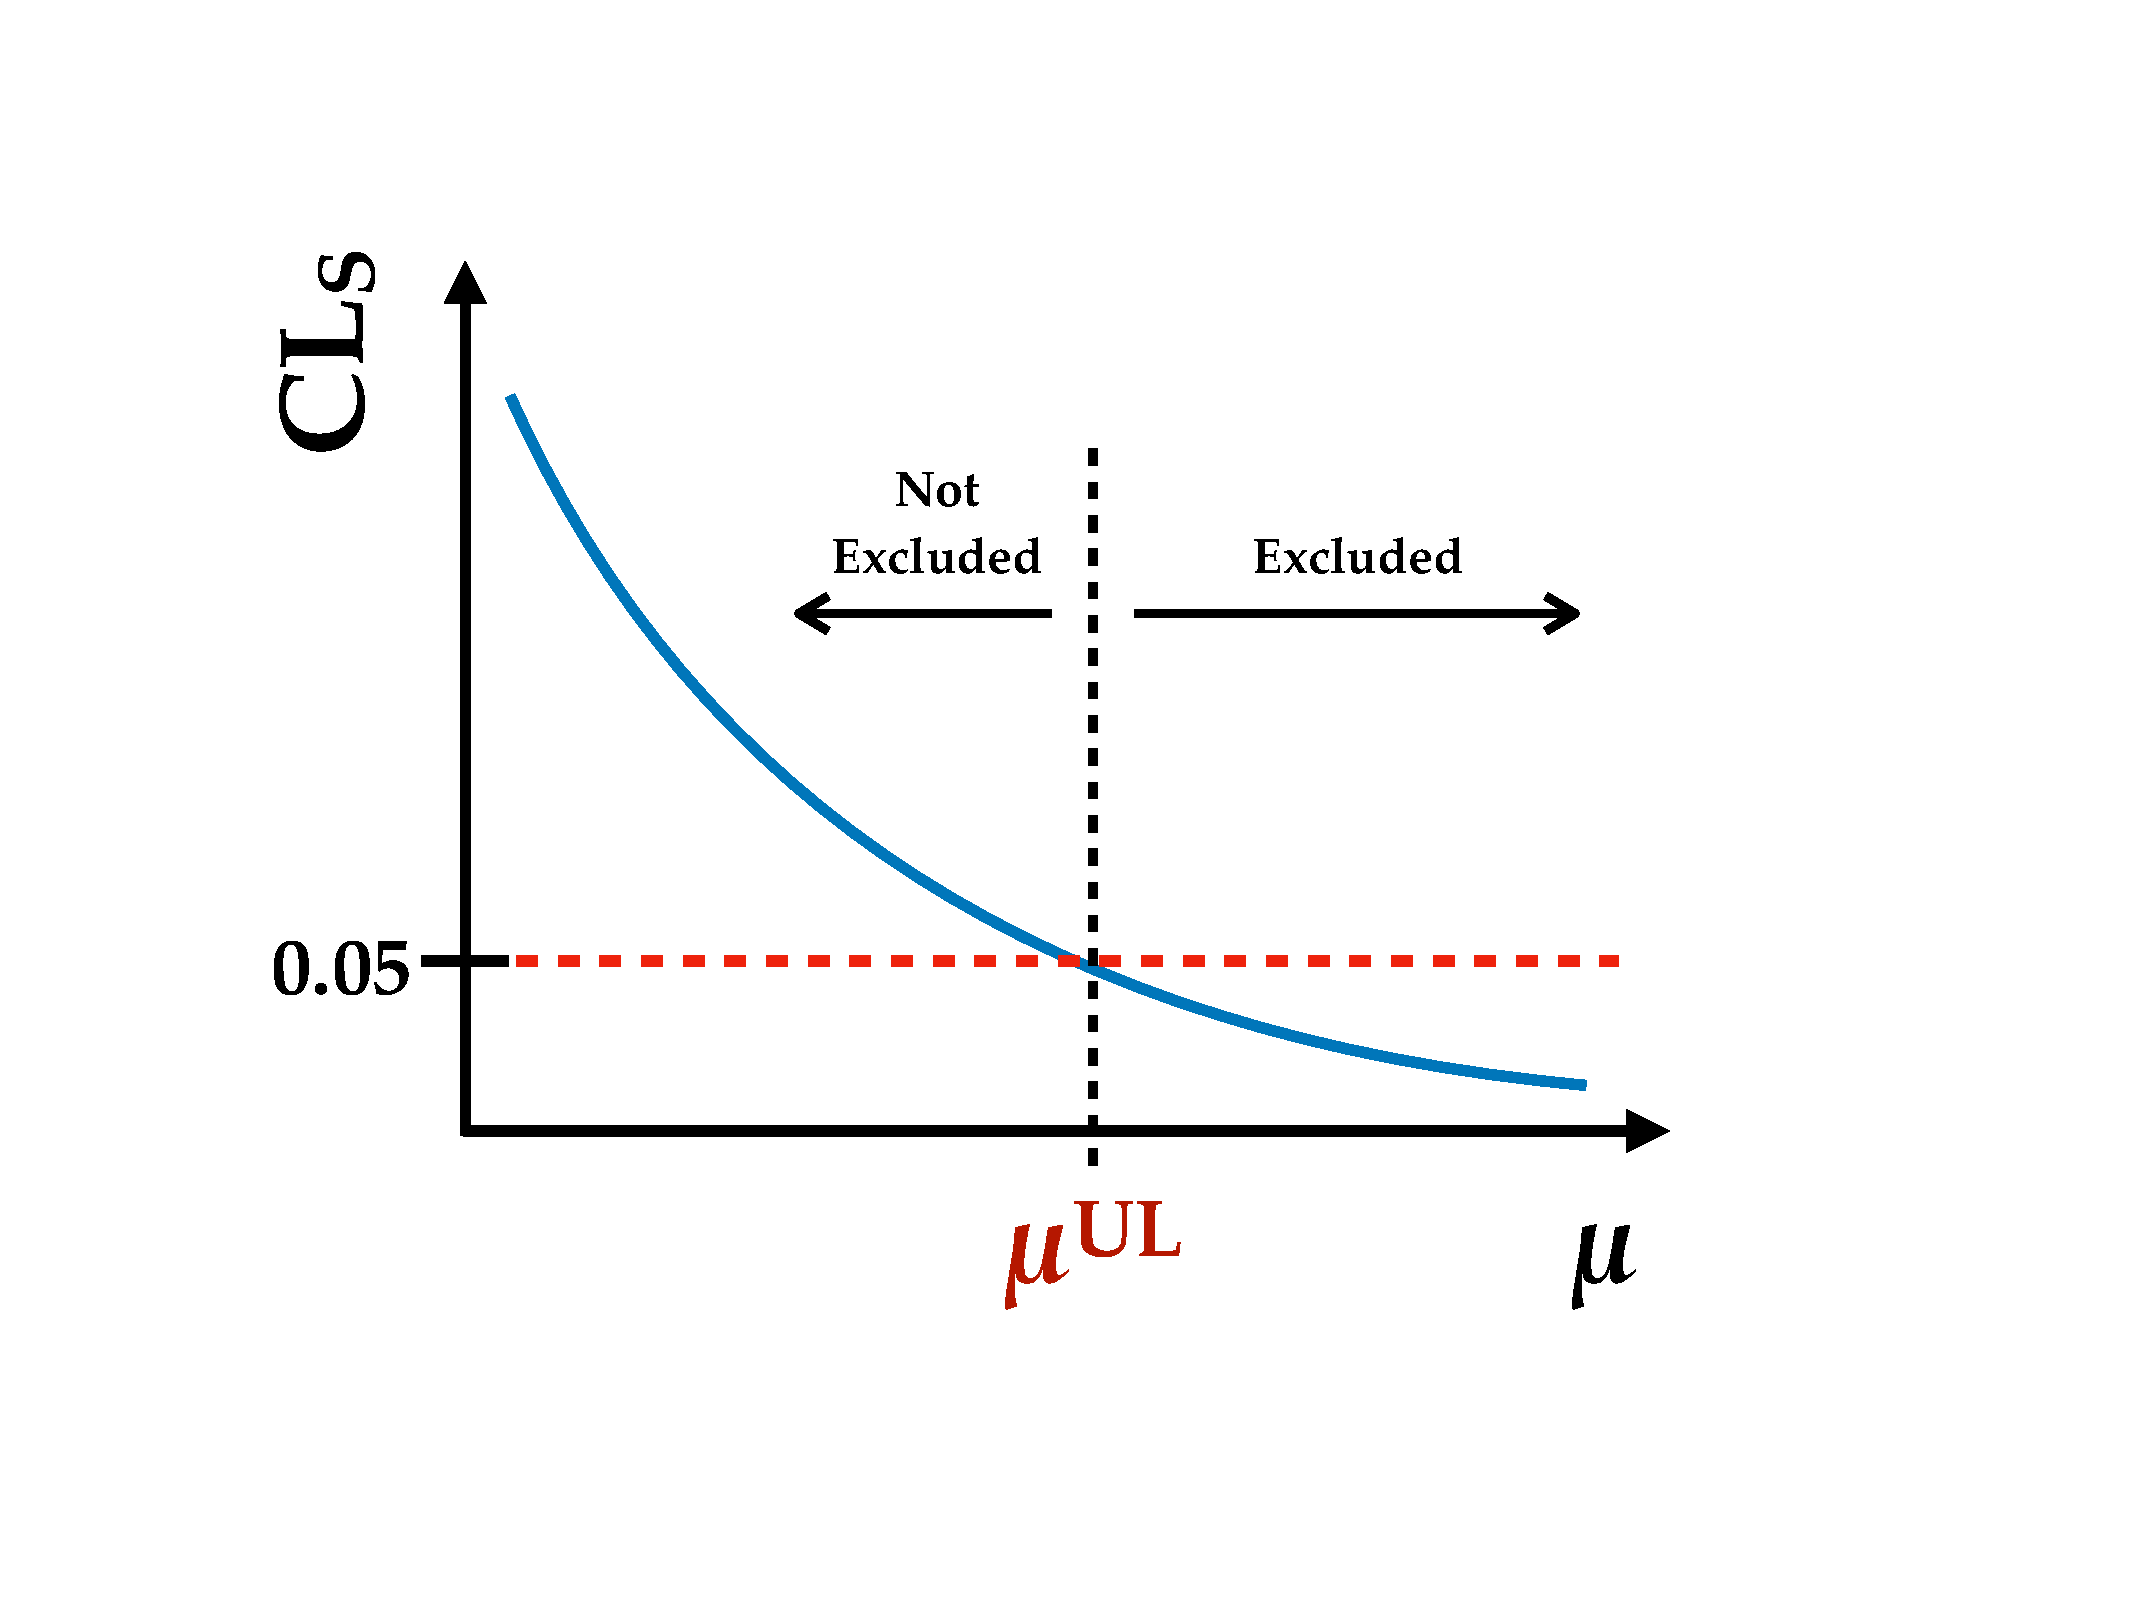
\includegraphics[width=0.5\textwidth]{figures/common_ana/stat_hypo/upper_limit_scan_examplePDF}
        \caption{
            An upper limit scan on the signal strength parameter $\mu$ associated with a signal hypothesis.
            The \cls, given by Equation~\ref{eq:cls_def}, is recomputed for a range of $\mu$ values
            describing a given signal hypothesis.
            This is shown by the blue line.
            The $\mu$ value at which the \cls curve crosses the line $\cls = 0.05$, $\mu^{\text{UL}}$, is the
            upper limit on $\mu$ for the signal hypothesis.
            Values of $\mu$ smaller than $\mu^{\text{UL}}$ remain compatible with the observed data,
            while those values greater than $\mu^{\text{UL}}$ are excluded at $95\%$ CL.
        }
        \label{fig:upper_limit_scan_cartoon}
    \end{center}
\end{figure}

%%%%%%%%%%%%%%%%%%%%%%%%%%%%%%%%%%%%%%%%%%%%%%%%%%%%%%%%%%%%%%%%%%%
%%%%%%%%%%%%%%%%%%%%%%%%%%%%%%%%%%%%%%%%%%%%%%%%%%%%%%%%%%%%%%%%%%%
%
% PROFILE LIKELIHOOD
%
%%%%%%%%%%%%%%%%%%%%%%%%%%%%%%%%%%%%%%%%%%%%%%%%%%%%%%%%%%%%%%%%%%%
%%%%%%%%%%%%%%%%%%%%%%%%%%%%%%%%%%%%%%%%%%%%%%%%%%%%%%%%%%%%%%%%%%%

\subsection{The Profile Likelihood Ratio Test Statistic}
\label{sec:likelihood}

The test statistic associated with many of the LHC experiments, including ATLAS,
and the one used in the analyses to be presented in Chapters~\ref{chap:search_stop} and
\ref{chap:search_hh} is based on a likelihood ratio.
The construction of the test statistic is described in this section.

In the analyses to be presented, so-called `counting experiments' are performed wherein
only the numbers of events, from data and the predicted background and signal,
are used as input.
These numbers are taken from all relevant regions in the analysis: the CRs and the SRs.
The expected number of events populating each region is given by the following:

\begin{align}
    N_r^\text{exp}(\mu_{\text{sig}}, \bm{\mu_{\text{bkg}}}, \bm{\theta}) = \mu_{\text{sig}} \cdot N_{r,\,\text{sig}}^{\text{exp}}(\bm{\theta}) + \sum\limits_{b\,\in \,\text{bkg}} \, \mu_b \cdot N_{r,\,b}^{\text{exp}}(\bm{\theta}),
    \label{eq:test_stat_n_r}
\end{align}
where $\bm{\theta}$ are a set of fit nuisance parameters (NP) associated with the systematic
uncertainties described in Section~\ref{sec:common_systematics},
$\bm{\mu_{\text{bkg}}}$ are normalisation factors associated with the background processes (indexed by `$b$'),
$\mu_{\text{sig}}$ is the signal-strength modifier associated with the signal hypothesis,
$N_{r,\,\text{sig}}^{\text{exp}}$ is the predicted signal yield in region $r$,
and $N_{r,\,b}^{\text{exp}}$ is the predicted background yield in region $r$ for process $b$.
The predicted number of events for each process, signal or background, depend on the $\bm{\theta}$ parameter vector
since systematic variations can adjust the overall normalisation of a given process or adjust
the acceptance of a given process in the phase space probed by the regions indexed by $r$.
Both of these effects result in a change in the predicted rate of a process in a given region.

The observed data yield in each region of the analysis is expected to obey Poisson statistics.
Therefore, the likelihood function $L(\mu_{\text{sig}}, \bm{\mu_{\text{bkg}}}, \bm{\theta})$ is
constructed as a product of Poisson probability terms:
\begin{align}
    L_0(\mu_{\text{sig}}, \bm{\mu_{\text{bkg}}}, \bm{\theta}) = \prod\limits_{r\,\in\,\text{regions}} \, 
            \frac
            {
                \left[N_r^{\text{exp}} ( \mu_{\text{sig}}, \bm{\mu_{\text{bkg}}}, \bm{\theta}) \right] ^ {N_r^{\text{obs}}}
            }
            {
                N_r^{\text{obs}}!
            }
            \cdot
            \exp\left[ N_r^{\text{exp}} ( \mu_{\text{sig}}, \bm{\mu_{\text{bkg}}}, \bm{\theta}) \right],
    \label{eq:likelihood_main}
\end{align}
where $N_r^{\text{obs}}$ is the observed data yield in region $r$.

{\color{red}{REORDER THIS TEXT}} It is standard practice to parametrize the systematic uncertainties associated with the measurements
of the $N_r^{\text{exp}}$ in such a way that $\bm{\theta} = 0$ (all of the $\theta_i$ equal to zero) corresponds to the central (nominal) value
of the set of parameters associated with the uncertainty (e.g. the nominal value of JES).
The values $\theta_i = \pm 1$ represent shifts in the parameter values by their $\pm 1\sigma$
variation, as defined by the systematic uncertainty (e.g. systematic shifts in the value of the JES).
The systematic uncertainties described in Section~\ref{sec:common_systematics} are typically
computed such that, at the level of performing a physics analysis, only the $\pm 1 \sigma$ shifts about the central value
in the associated parameter are known.
Means of interpolation and extrapolation, needed to obtain a smoothly varying response in the
numbers of predicted events as the $\theta$ parameters vary continously between their $\pm 1 \sigma$ values,
are provided by the \textsc{HistFactory} toolkit~\cite{HistFactory}.
The effects of the NP associated with each of the analysis' systematic uncertainties
are implemented as \textit{constraint terms} in the likelihood appearing in Equation~\ref{eq:likelihood_main}.
These terms are typically implemented as Gaussians centered on zero and with a width of 1:
%are implemented as Gaussian \textit{constraint terms}, with wi in the likelihood defined in Equation~\ref{eq:likelihood_main}:
\begin{align}
    L(\mu_{\text{sig}}, \bm{\mu_{\text{bkg}}}, \bm{\theta}) = L_0(\mu_{\text{sig}}, \bm{\mu_{\text{bkg}}}, \bm{\theta})
        \, \cdot \, \prod\limits_{i = 1}^{n} \frac{1}{\sqrt{2 \pi}} \, \exp \left( - \frac{\theta_i^2}{2} \right).
    \label{eq:full_likelihood}
\end{align}
%The constraint terms represent Gaussians centered on 0 and with a width of 1.
%This is equivalent to:
%\begin{align}
%    \theta^{\prime} = \frac{ \theta - \hat{\theta} } {\sigma},
%\end{align}
%allowing for the post-fit NP to be easily compared with the pre-fit ones in the following manner.
%A post-fit value and uncertainty of the NP near 0 and 1, respectively, indicate that the data
The best estimates (maximum likelihood estimates, MLE) for the parameters ($\mu_{\text{sig}}$, $\bm{\mu_{\text{bkg}}}$, $\bm{\theta}$)
are determined in the fit to the observed data, $\bm{N^{\text{obs}}}$, via the maximization
of the likelihood function given by Equation~\ref{eq:full_likelihood}. 
Typically, and equivalently, the negative log likelihood, $-\ln L$, is minimized.
Technically, the minimization of Equation~\ref{eq:full_likelihood} in the analyses to be presented
in Chapters~\ref{chap:search_stop} and \ref{chap:search_hh} is done using \textsc{Miniuit}
via an interface provided by \textsc{RooFit}~\cite{MINUIT,RooFitI}.
The values of all parameters prior to (after) the minimization procedure are referred to as the
`pre-fit' (`post-fit') values.
The pre-fit values for the $\mu_{\text{bkg}}$ parameters are set to 1 and the $\theta_i$ are set to $0$, corresponding
to the central values of the Gaussian-shifted parameters associated with the systematic uncertainties.

The test statistic defined for the analyses to be presented is based on the following
\textit{profile likelihood ratio},
\begin{align}
    \lambda(\mu_{\text{sig}}) \equiv
        \frac{
            L(\mu_{\text{sig}}, \hat{\hat{\bm{\mu}}}_{\text{bkg}}, \hat{\hat{\bm{\theta}}})
        }
        {
            L(\hat{\mu}_{\text{sig}}, \hat{\bm{\mu}}_{\text{bkg}}, \hat{\bm{\theta}})
        },
    \label{eq:likelihood_ratio}
\end{align}
where in the numerator the parameters $(\bm{\mu}_{\text{bkg}}, \bm{\theta})$ are fit to their MLE values
for a given value of the assumed value of the signal-strength parameter $\mu_{\text{sig}}$.
In the denominator, the full set of parameters ($\mu_{\text{sig}}$, $\bm{\mu_{\text{bkg}}}$, $\bm{\theta}$) are
equal to their MLE values.
The likelihood ratio defined in Equation~\ref{eq:likelihood_ratio} is used to define the
final test statistic relevant to the analyses,
\begin{align}
    q_{\mu_{\text{sig}}} = - 2 \ln \lambda (\mu_{\text{sig}}),
    \label{eq:pll_test_stat}
\end{align}
which is used to perform the hypothesis tests described in Section~\ref{sec:hypo_test}.

\subsubsection{Profile Likelihood Fit Determination of Background Constraints}

We note here that the quantites described by $\bm{\mu_{\text{bkg}}}$ in Equations~\ref{eq:test_stat_n_r}--\ref{eq:pll_test_stat} correspond to normalisation correction
factors for a given SM background process.
In the analyses to be presented in Chapters~\ref{chap:search_stop} and \ref{chap:search_hh},
for the background processes for which a dedicated CR is not defined, the associated $\mu_b$ are
set to 1 and are not allowed to vary during the fit (i.e. their pre-fit and post-fit values are equal).
%these values are set to one for all background processes that do not have a dedicated
%CR and are not allowed to vary from this value during the fit procedure.
For those processes for which a dedicated CR is defined, the associated $\mu_b$ parameters
are analogous to the normalisation correction factors described in Section~\ref{sec:control_region_method} and
are unconstrained in the fit procedure.
They are therefore said to `freely float' during the fit and 
their post-fit value does not necessarily correspond to their pre-fit one.
Given the low numbers of events typically expected in the SRs, and the relatively
large numbers and purities expected in the CRs, the post-fit values of the $\mu_b$ typically
correspond to those values expected from the simple computations provided by Equation~\ref{eq:mu_fac}
and/or Equation~\ref{eq:mu_fac_expand}.
An additional note is that in the signal-plus-background hypotheses with $\mu_{\text{sig}} \ne 0$, if
the CRs have a non-negligible contamination of signal events, however, this correspondence will generally not be true
since the post-fit values of the $\mu_b$ will depend on a given value of the $\mu_{\text{sig}}$ parameter.
The desire to construct a robust background-only model is one of the motivating factors, then,
in designing analyses in such a way as to minimize the signal contamination in the CRs.

\subsubsection{Profiling}
\label{sec:profiling}

The Gaussian constraint terms in Equation~\ref{eq:full_likelihood}, centered on 0 and with widths of 1,
are equivalent to transforming the $\bm{\theta}$ parameters associated with the systematic uncertainties as follows,
\begin{align}
    \bm{\theta}^{\prime} = \frac{\bm{\theta} - \bm{\hat{\theta}}}{\bm{\hat{\sigma}}},
    \label{eq:theta_gaus}
\end{align}
where the quantity $\bm{\sigma}$ corresponds to the initial widths of the $\pm 1 \sigma$ variations
associated with the systematic variation represented by $\bm{\theta}$.
Equation~\ref{eq:theta_gaus} normalises all NP to facilitate the easy comparison of their pre- and post-fit values and uncertainties.
For a given NP, then, a post-fit value and uncertainty near 0 and 1, respectively, indicate
that the data was not able to adjust the NP.
Changes in the post-fit NP values (uncertainties) are referred to as NP `pulling' (`profiling').
NP values may be pulled far from zero in order to maximize the overall agreement of the background prediction
with data during the fit procedure.
NP may be profiled in such a way that the post-fit uncertainties on the NP are smaller than the
the initial estimate of the uncertainty provided by auxiliary measurements and data.
Such a case indicates that the initial prior on the impact of the systematic uncertainty was too
large and that the uncertainties may be reduced so as to be more compatible  with the range allowed by
the data statistics relevant for the analysis at hand.
This potential for the profiling mechanism to reduce the overall impact of systematic uncertainties
on an analysis' results is seen as a general benefit of the profile likelihood prescription described
by Equations~\ref{eq:likelihood_ratio} and \ref{eq:pll_test_stat}.
The interpretation of this is that the profiling mechanism allows for the impact of the systematic uncertainties
to be more accurately characterised in the phase space in which they are being applied, as opposed
to that of the auxiliary measurements in which they are initially derived.


\subsection{Toy Examples of the Profile Likelihood Fit}
\label{sec:profile_examples}

The best way to get a feel for the profiling mechanisms just described is via a few simple
examples, to which we turn now.

\subsubsection{Profile Likelihood Fit Example 1a}
\label{sec:profiling_example_1a}

This example illustrates the mechanisms of both NP profiling and pulling.
We set up a dummy analysis, with two regions and two backgrounds only.
The regions are referred to as `Region 1' and `Region 2' and the backgrounds
are `Bkg 1' and `Bkg 2'.
A summary of the predicted and observed yields, as well as the uncertainties on
the predicted yields, is as follows:

\begin{itemize}
    \item \underline{\textbf{Region 1}}
        \begin{itemize}
            \item Background composition: 80 events from Bkg 1
            \item Observed data: 100 events
            \item Systematic Uncertainties:
            \begin{itemize}
                \item `Norm. Bkg. 1': A 50\% systematic uncertainty on the predicted yield of Bkg 1
            \end{itemize}
        \end{itemize}
    \item \underline{\textbf{Region 2}}
        \begin{itemize}
            \item Background composition: 100 events from Bkg 2
            \item Observed data: 100 events
            \item Systematic Uncertainties:
            \begin{itemize}
                \item `Norm. Bkg. 2$_1$': A 10\% systematic uncertainty on the predicted yield of Bkg 2
                \item `Norm. Bkg. 2$_2$': An additional 10\% systematic uncertainty on the predicted yield of Bkg 2
            \end{itemize}
        \end{itemize}
\end{itemize}

From this information, a likelihood as described by Equation~\ref{eq:full_likelihood} is constructed.
In this setup, all of the $\mu$ parameters are set to 1 for the backgrounds
and NP constraint terms parametrized by $\theta$ terms
for each of the three uncertainties are included.
The pre-fit situation is illustrated by the left side of Figure~\ref{fig:prof_ex_1_np50}.
A profile-likelihood fit to the observed data is performed and the results for the fitted parameters
are shown in Figure~\ref{fig:prof_ex_1_pulls} and by the
right side of Figure~\ref{fig:prof_ex_1_np50}.

Focusing first on Region 1, we see that after the fit the pre-fit 20 event excess is removed by
the increase in Bkg. 1's predicted yield.
This is explained by the NP on Bkg. 1 being pulled by nearly 0.5, as seen in Figure~\ref{fig:prof_ex_1_pulls}.
Using Equation~\ref{eq:theta_gaus}, a pull by 0.5 in this NP is precisely 20 events ($\theta^{\text{post-fit}} \times ( \text{pre-fit uncertainty} \times N^{\text{pre-fit}}) \rightarrow 0.5 \times (0.5 \times 80) = 20$).
The post-fit uncertainty has also been reduced to that allowed by the data statistics, which is driven
by the NP on Bkg. 1 being profiled from its initial uncertainty of $\pm 1$ to $\pm 0.25$ ($\Delta \theta^{\text{post-fit}} \times (\text{pre-fit uncertainty} \times N^{\text{pre-fit}}) \rightarrow 0.25 \times (0.5 \times 80) = 10$), also seen in Figure~\ref{fig:prof_ex_1_pulls}.

Looking to the post-fit results of Region 2, we see that, as with Region 1, the overall
background uncertainty has been profiled so as to be compatible with that allowed by the data statistics.
The main difference with respect to Region 1, however, is the fact that there are two NP constraints
on Bkg. 2.
Each of the NP constraint terms is already at the level of $10\%$ that corresponds to the data statistics.
There is therefore a redundancy in the NP constraints on Bkg. 2 and the fit develops a correlation between
them such that their combined post-fit impact on Bkg. 2 is as seen on the right side of Figure~\ref{fig:prof_ex_1_np50}.
The correlation between the two constraints is seen in Figure~\ref{fig:prof_ex_1_pulls} to be $\rho = -0.5$,
which, in this simple scenario, can be expected to be the case by the following:
\begin{align}
    \sigma_{1} &= \sigma_{2} = \sigma, \nonumber \\
    \sigma_{1 \oplus 2} &= \sqrt{ \sigma_1^2 + \sigma_2^2 + 2 \sigma_1 \sigma_2 \rho } = \sigma, \nonumber
\end{align}
where, in the second line, we expect $\sigma$ to be at the level of the data statistics.
This requires $\rho = -0.5$ and is indeed what the profile-likelihood fit ends up with.

\begin{figure}[!htb]
    \begin{center}
        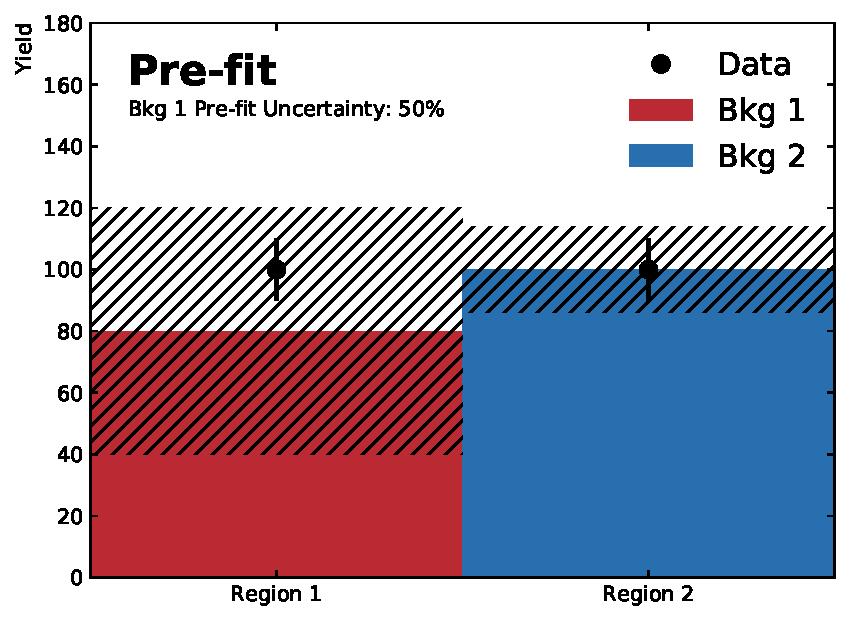
\includegraphics[width=0.48\textwidth]{figures/common_ana/stat_hypo/profile_examples/profile_ex_1_NP50_pre}
        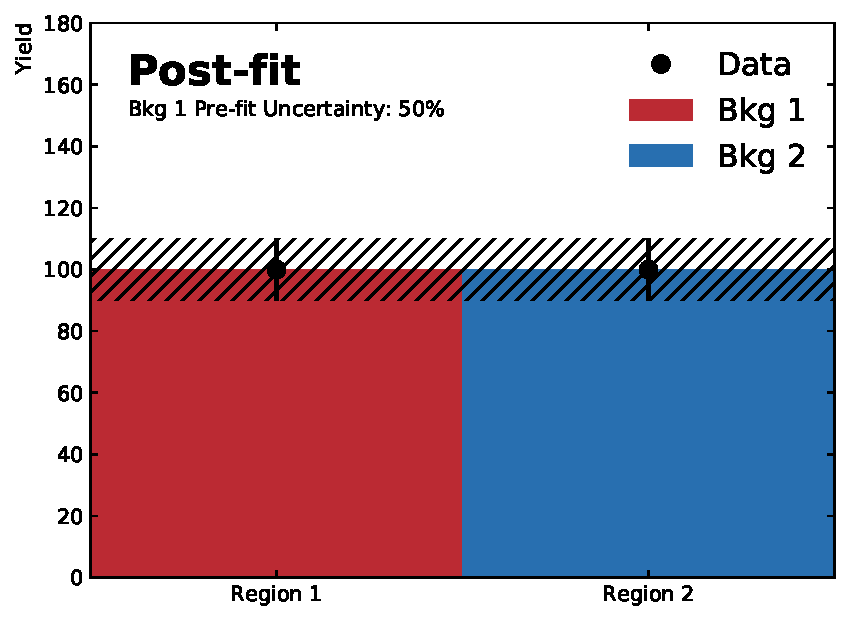
\includegraphics[width=0.48\textwidth]{figures/common_ana/stat_hypo/profile_examples/profile_ex_1_NP50_post}
        \caption{
            \textbf{\textit{Left}}: Pre-fit scenario for Example 1a, described in the text.
            \textbf{\textit{Right}}: Post-fit scenario for Example 1a, described in the text.
        }
        \label{fig:prof_ex_1_np50}
    \end{center}
\end{figure}

\begin{figure}[!htb]
    \begin{center}
        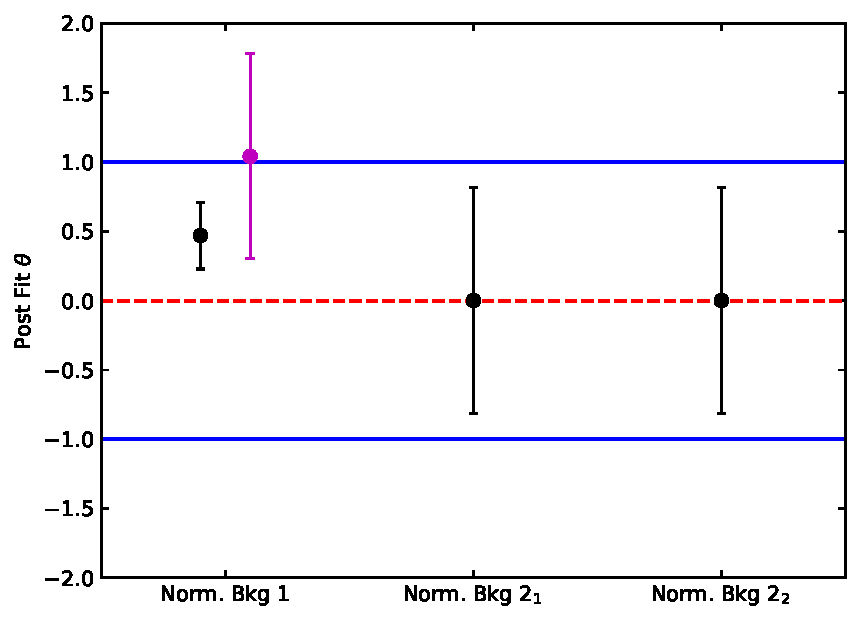
\includegraphics[width=0.48\textwidth]{figures/common_ana/stat_hypo/profile_examples/profile_ex_1_pulls}
        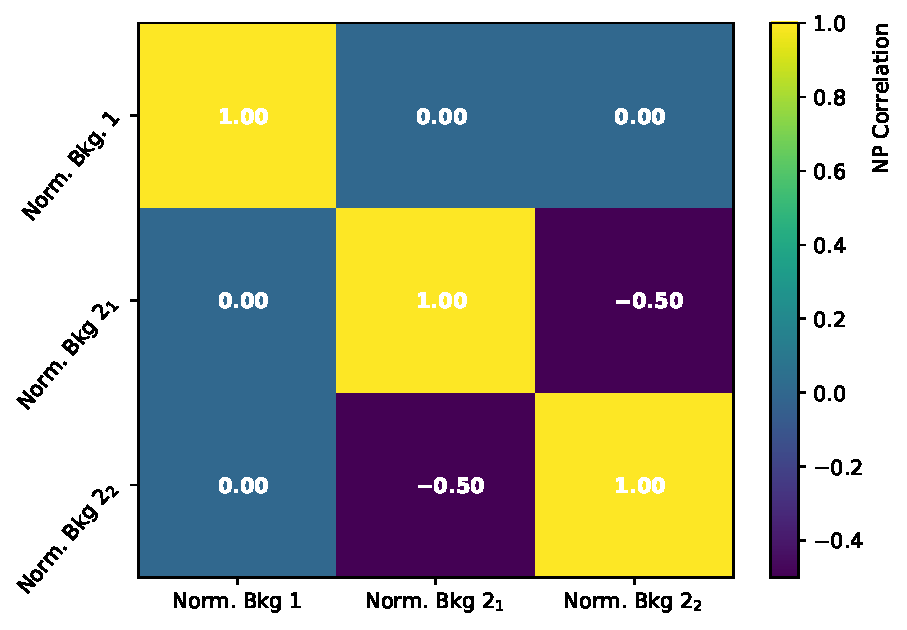
\includegraphics[width=0.48\textwidth]{figures/common_ana/stat_hypo/profile_examples/np_corr_ex_1}
        \caption{
            \textbf{\textit{Left}}: Post-fit values for the parameters entering the profile-likelihood fit
                described in the text. The post-fit result for the NP `Norm. Bkg. 1' in pink corresponds
                to that of the fit configuration described in Example 1b, below.
                All other parameters (in black) correspond to those in the fit configuration described in Example 1a.
            \textbf{\textit{Right}}: Post-fit correlation matrix for the parameters entering the profile-likelihood
                fit described in the text.
        }
        \label{fig:prof_ex_1_pulls}
    \end{center}
\end{figure}

\subsubsection{Profile Likelihood Fit Example 1b}
\label{sec:profiling_example_1b}

In the previous example we saw that, through the pulling of a constraint term,
the complete removal of a discrepancy between the observed data and the
predicted background was made possible.
This reinforces the idea that the predicted numbers of events are dependent
upon the NP entering the fit ($N^{\text{exp}} \rightarrow N^{\text{exp}}(\bm{\theta})$)
and that their post-fit values can change even if their is no explicit normalisation-correcting $\mu$ terms in the fit.
Of course, the large uncertainty on Bkg. 1's prediction in Example 1a equates to a loose constraint term and allows for a large degree of
flexibility in the fit for it to be pulled in such a way as to have the post-fit prediction perfectly line up with
the data being fit to.
In this current example we reproduce the fit configuration introduced in Example 1a, but instead the
uncertainty on Bkg. 1 in Region 1 is reduced to $10\%$.
The pre- and post-fit distributions of the observed and predicted events, with their uncertainties,
are shown in Figure~\ref{fig:prof_ex_1_np10}.
The results of the fit for Region 2 are exactly the same as in Example 1a since we have not altered
the parameters describing this region.

Given the tighter constraint on the predicted yield of Bkg. 1 in Region 1, as compared to Example 1a,
the NP describing Bkg. 1's normalisation uncertainty does not have enough freedom to be pulled to fully
cover the 20 event excess.
The post-fit value of the NP is shown in pink in Figure~\ref{fig:prof_ex_1_pulls}.
It is pulled to a value of 1.04, which corresponds to just above 8 events as seen in Figure~\ref{fig:prof_ex_1_np10}.
The smaller uncertainty Bkg. 1's prediction in this example, as compared to Example 1a, corresponds
to a higher level of confidence in its pre-fit value.
The associated NP constraint term, therefore, should not be allowed the freedom to contradict this
high degree of confidence by shifting the prediction to the same extent as that in Example 1a.
%This is unlike the case of Example 1a,
%where there was relatively little confidence in the pre-fit prediction of Bkg. 1.

\begin{figure}[!htb]
    \begin{center}
        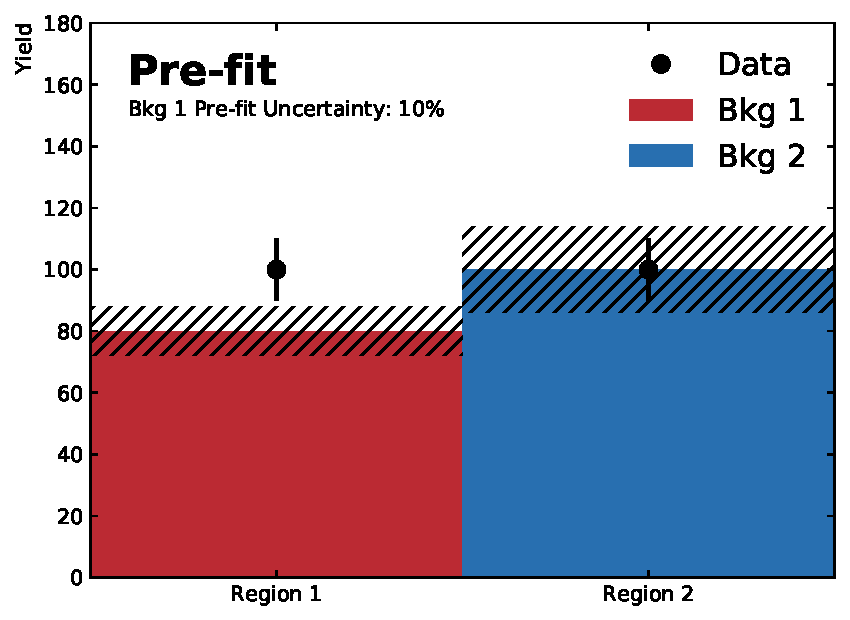
\includegraphics[width=0.48\textwidth]{figures/common_ana/stat_hypo/profile_examples/profile_ex_1_NP10_pre}
        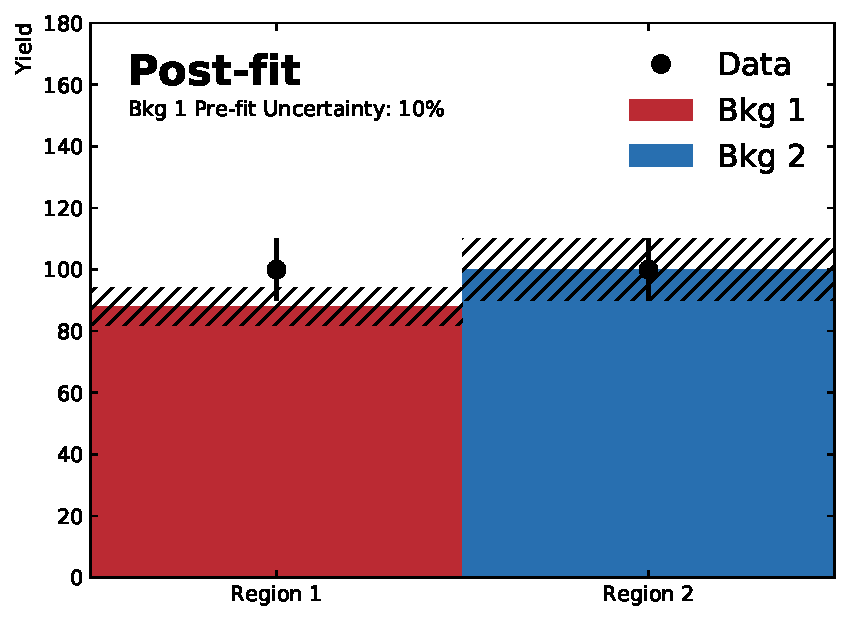
\includegraphics[width=0.48\textwidth]{figures/common_ana/stat_hypo/profile_examples/profile_ex_1_NP10_post}
        \caption{
            \textbf{\textit{Left}}: Pre-fit scenario for Example 1b, described in the text.
            \textbf{\textit{Right}}: Post-fit scenario for Example 1b, described in the text.
        }
        \label{fig:prof_ex_1_np10}
    \end{center}
\end{figure}

\subsubsection{Profile Likelihood Fit Example 2}
\label{sec:profiling_example_2}

In this example we again set up the same fit configuration as in Example 1a.
However, an additional process, `Bkg. $\mu$', with 20 events predicted in Region 1 is added.
A freely floating normalisation correction term is added to the fit,
associated with this newly added background (hence its name).
Again, a profile-likelihood fit to the observed data is run.
The pre- and post-fit distributions of the observed data and predicted backgrounds,
with their uncertainties, are shown in Figure~\ref{fig:prof_ex_2_pre}.

From the post-fit distributions shown in Figure~\ref{fig:prof_ex_2_pre}, we see the
expected result that the post-fit uncertainties on the predicted backgrounds
are such that they match the precision allowed by the data statistics.
As we have not changed anything in Region 2, relative to Example 1a and Example 1b,
we do not expect the post-fit values of the NP associated with Bkg. 2 to have changed relative
to those examples.
The post-fit value of the NP associated with Bkg. 1, however, differs quite substantially
relative to the earlier examples, as is seen in Figure~\ref{fig:prof_ex_2_pulls}.
We see that the NP term `Norm. Bkg. 1' is neither pulled nor profiled.
Instead, the unconstrained $\mu$ parameter associated with Bkg. 1 is able to `eat up'
the remaining degrees of freedom needed for the reduction in the background prediction's uncertainty.
Since the pre-fit predicted yield of Bkg. $\mu$ is such that the complete background
prediction in Region 1 matches the data, the post-fit value for the $\mu$ term is equal to its
pre-fit value of 1.
It's uncertainty, however, is $\pm 1.90$ and corresponds to a post-fit uncertainty
on Bkg. $\mu$'s prediction of nearly 40 events ($1.90 \times 20$).
This precision on Bkg. $\mu$ matches that of Bkg. 1, with its predicted 80 events
with 50\% uncertainty.
This illustrates the fact that the $\mu$ term is completely degenerate with the NP associated with Bkg. 1:
any variation in the NP term can be fully compensated by the unconstrained $\mu$ term.
This is illustrated in the right side of Figure~\ref{fig:prof_ex_2_pulls},
% the post-fit
%correlation between Bkg. 1's NP constraint and $\mu$ terms,
where it can be seen that Bkg. 1's NP constraint and $\mu$ terms exhibit almost perfect anti-correlation.

\begin{figure}[!htb]
    \begin{center}
        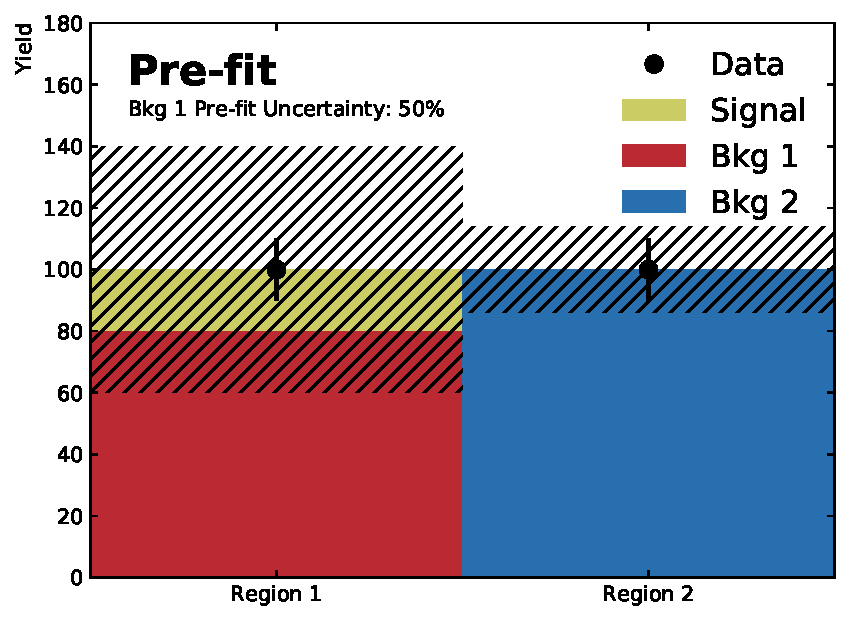
\includegraphics[width=0.48\textwidth]{figures/common_ana/stat_hypo/profile_examples/profile_ex_2_pre}
        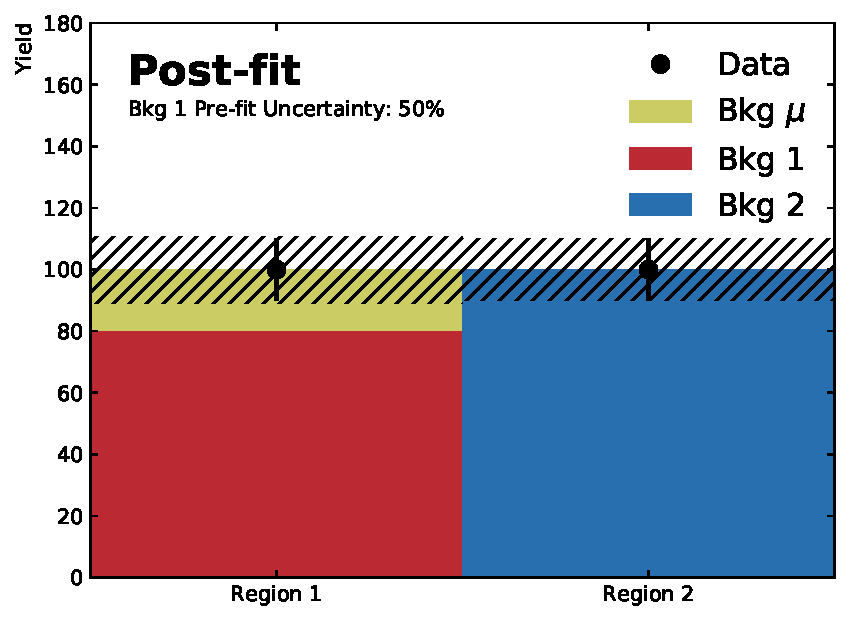
\includegraphics[width=0.48\textwidth]{figures/common_ana/stat_hypo/profile_examples/profile_ex_2_post}
        \caption{
            \textbf{\textit{Left}}: Pre-fit scenario for Example 2, described in the text.
            \textbf{\textit{Right}}: Post-fit scenario for Example 2, described in the text.
        }
        \label{fig:prof_ex_2_pre}
    \end{center}
\end{figure}

\begin{figure}[!htb]
    \begin{center}
        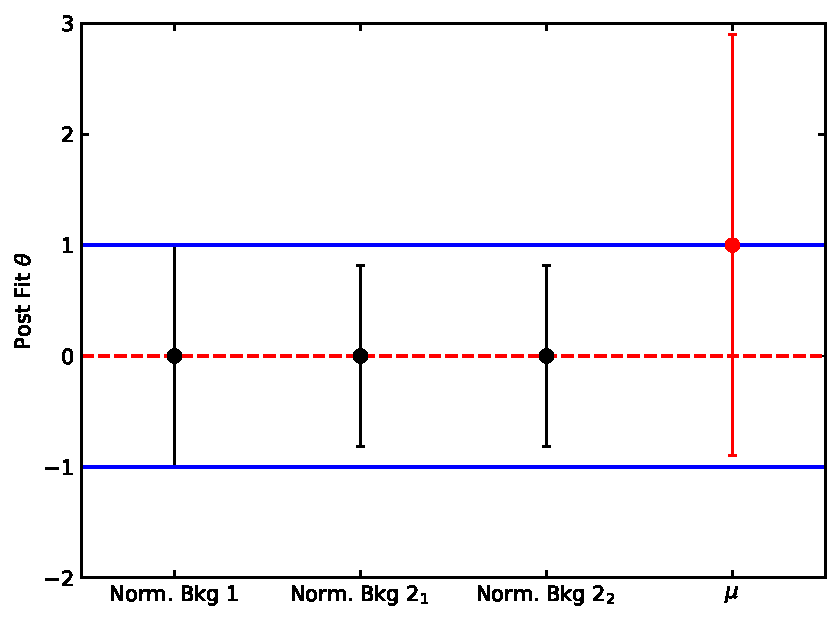
\includegraphics[width=0.48\textwidth]{figures/common_ana/stat_hypo/profile_examples/profile_ex_2_pulls}
        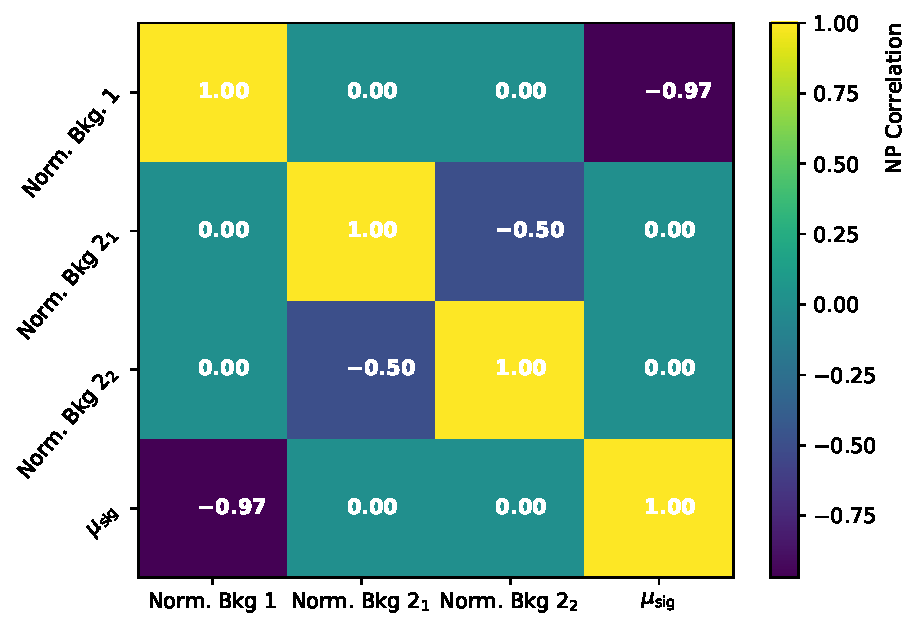
\includegraphics[width=0.48\textwidth]{figures/common_ana/stat_hypo/profile_examples/np_corr_ex_2}
        \caption{
            \textbf{\textit{Left}}: Post-fit values for the parameters entering the profile-likelihood fit
                of Example 2,
                described in the text. 
            \textbf{\textit{Right}}: Post-fit correlation matrix for the parameters entering the profile-likelihood
                fit of Example 2, described in the text.
        }
        \label{fig:prof_ex_2_pulls}
    \end{center}
\end{figure}

It is interesting to make note of the fact, exemplified by the above discussion, that the precision on a given process' $\mu$ term,
if allowed to vary in the fit, is highly dependent on the precision of the prediction of the
other backgrounds.
This, of course, is intuitive and has meaningful consequences for searches for new physics, in which the signal-plus-background
hypotheses are characterised by $\mu_{\text{sig}}$ terms associated with the sought-for signal processes.
Large uncertainties in background predictions result in less precise statements about the presence
of signal in the analyses' regions.
This, then, reduces the statistical power (c.f. Equation~\ref{eq:power_level}) of the hypothesis tests
being performed and, if the uncertainties are large enough, prevent the analyses from making meaningful
statements about the compatibility of the signal-plus-background hypotheses with the observed data.

As an illustration, Figure~\ref{fig:cls_scan_uncert} shows the CL$_s$ computed as a function of varying signal-to-background ratio, for several background uncertainty hypotheses,
for a fixed number of predicted background and data events in a single-region analysis.
%This is shown in Figure~\ref{fig:cls_scan_uncert}, 
%The scenario shown in Figure~\ref{fig:cls_scan_uncert} is not unlike those to be
%presented in Chapters~\ref{chap:search_stop} and \ref{chap:search_hh}, in which the predicted
%and observed event counts are relatively low.
The number of signal events needed to cross the critical CL$_s <0.05$ region
at which a signal hypothesis may be considered excluded is quite sensitive to the uncertainty
on the background prediction.
Again, this is intuitive mainly from the perspective that reduced levels of precision
in the background prediction correspond directly to increased levels of ambiguity 
as to the point at which a signal becomes apparent.

Figure~\ref{fig:cls_scan_uncert} also illustrates the increase in the upper limit
on a signal process' cross-section, as a result of increased background uncertainty,
in cases where no excess in data is observed.
For example, imagine that the sought-for signal process has a predicted cross-section leading to an
$S/B$ value of 0.4 in Figure~\ref{fig:cls_scan_uncert}.
At a level of background uncertainty of $30\%$, with a CL$_s \approx 0.35$, this process can neither be said
to be excluded nor to actually exist.
At this background uncertainty, the analysis would find an upper-limit on the signal process' $\mu_{\text{sig}}$ term nearing a value of 2,
since the CL$_s$ crossing point is near $S/B = 0.8$.
%only be sensitive to the type of process
%described by the sought-for signal if it had a cross-section nearly twice that of the predicted
%one, since the CL$_s$ crossing point is near $S/B = 0.8$.
Using this terminology, then, when no discrepancies between the predicted background and observed event counts
are seen, the upper-limit value under the hypothesis for a
given signal process
quantifies the analysis'
sensitivity to that process.
If the upper-limit value is $200$ times the predicted cross-section, the analysis is not sensitive to the process at all.
However, if the upper-limit value is $\mathcal{O}(1)$ times the predicted process' cross-section, the analysis
is nearing the regime in which meaningful statements about the existence of that process, at its predicted cross-section, can begin to be made.
If an upper-limit value corresponds to a cross-section value that is \textit{less} than the predicted one,
the process --- as predicted --- is excluded.
%Thinking in these terms is relevant to the search presented in Chapter~\ref{chap:search_hh},
%in which a search for Standard Model Higgs boson pair production is presented.

\begin{figure}[!htb]
    \begin{center}
        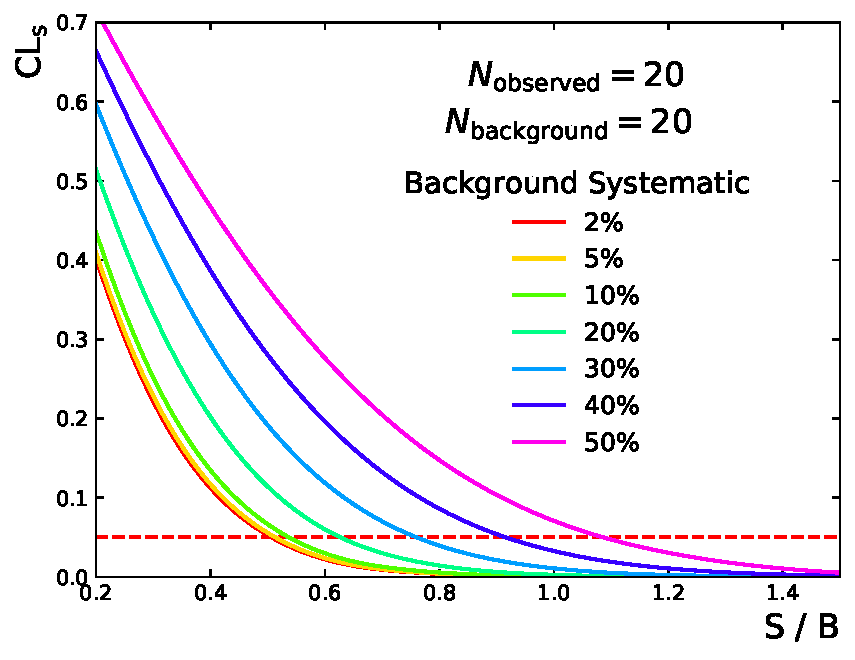
\includegraphics[width=0.6\textwidth]{figures/common_ana/stat_hypo/cls_bkguncert_scan}
        \caption{
            Dependence of computed CL$_s$ on the signal-to-background ratio for a single-region
            analysis in which 20 events are predicted and 20 events are observed, shown
            for varying levels of uncertainty on the predicted background.
        }
        \label{fig:cls_scan_uncert}
    \end{center}
\end{figure}

\FloatBarrier
\subsection{Asymptotic Formulation of Likelihood Ratio Tests}

{\color{red}{Describe the asympotitc formula used for the analysis to be presented and illustrate
examples of how various p values are obtained, as well as how analysis sensitivity is optimized}}


%%%%%%%%%%%%%%%%%%%%%%%%%%%%%%%%%%%%%%%%%%%%%%%%%%%%%%%%%%%%%%%%%%%%%%
%%%%%%%%%%%%%%%%%%%%%%%%%%%%%%%%%%%%%%%%%%%%%%%%%%%%%%%%%%%%%%%%%%%%%%
%
% FAKES
%
%%%%%%%%%%%%%%%%%%%%%%%%%%%%%%%%%%%%%%%%%%%%%%%%%%%%%%%%%%%%%%%%%%%%%%
%%%%%%%%%%%%%%%%%%%%%%%%%%%%%%%%%%%%%%%%%%%%%%%%%%%%%%%%%%%%%%%%%%%%%%
\section{Estimation of Sources of Fake and Non-prompt Leptons}
\label{sec:fakes}

Despite both the high levels of accuracy achieved by the ATLAS simulation
infrastructure and the lepton reconstruction and identification algorithms
described in Chapter~\ref{chap:objects}, sources of misidentified reconstructed
leptons still exist and lead to an additional source of backgrounds to
the analyses discussed in Chapters~\ref{chap:search_stop} and \ref{chap:search_hh}.
These background sources of leptons are broken down into two categories:
\begin{itemize}
    \item \textbf{Fake leptons}: Cases in which signals in the ATLAS detector
        are selected as being leptons when in fact there is no real lepton present
    \item \textbf{Non-prompt leptons}: When real, genuine leptons are identified
        but they are not leptons originating from the primary $pp$ hard-scatter interaction process
        of interest
\end{itemize}
In the subsequent discussion, the term `fake' will be used in reference to the two
categories listed above, unless specified otherwise.

The contribution of backgrounds leading to sources of fake leptons are generally predicted
using methods based on the observed data --- referred to as `data-driven' methods ---
and arise from various sources and mechanisms.
The sources of fake leptons will be described in Section~\ref{sec:fake_lepton_sources}, separately for
electrons and muons.
Section~\ref{sec:fake_dd_motivation} provides some reasoning for why a data-driven
approach is generally taken for estimating these backgrounds.
Sections~\ref{sec:matrix_method} and \ref{sec:same_sign_extrap} go on to describe
the two data-driven approaches taken in the analyses to be presented in this thesis
for estimating fake lepton contributions: the so-called `Matrix Method' and the `Same-sign Extrapolation Method', respectively.

%%%%%%%%%%%%%%%%%%%%%%%%%%%%%%%%%%%%%%%%%%%%%%%%%%%%%%%%%%%%%%%%%%%
%%%%%%%%%%%%%%%%%%%%%%%%%%%%%%%%%%%%%%%%%%%%%%%%%%%%%%%%%%%%%%%%%%%
%
% SOURCES OF FAKE LEPTONS
%
%%%%%%%%%%%%%%%%%%%%%%%%%%%%%%%%%%%%%%%%%%%%%%%%%%%%%%%%%%%%%%%%%%%
%%%%%%%%%%%%%%%%%%%%%%%%%%%%%%%%%%%%%%%%%%%%%%%%%%%%%%%%%%%%%%%%%%%
\subsection{Sources of Fake Leptons}
\label{sec:fake_lepton_sources}

The types and sources of fake leptons generally have different experimental signatures
than those leptons that genuinely originate from the $pp$ hard-scatter.
However, due to the non-perfect lepton identification and isolation algorithms,
such sources are able to contaminate the various regions of an analysis.
The rates of contamination are generally quite low for the analyses to be presented, but their inclusion in the background
estimates of the analyses has measurable consequences nevertheless.

The analyses to be presented in the current thesis make use of $b$-tagging algorithms
to identify jets originating from $b$-hadrons.
Fake leptons, both electrons and muons, can originate from the semi-leptonic decays of
$b$- and $c$-quarks within these $b$-tagged jets, following $b\rightarrow \ell$ or cascade-type
$b \rightarrow c \rightarrow \ell$ decays of the $B$ hadrons within the jets.
The leptons resulting from such decays are typically embedded within or very close to
the originating reconstructed jet object and the lepton isolation requirements
are intended to reduce this type of background.
The subsequent paragraphs will describe additional sources of fake electrons
and muons, which generally differ between the two lepton species.

%%%%%%%%%%%%%%%%%%%%%%%%%%%%%%%%%%%%%%%%%%%%%%%%%%%%%%%%%%%%%%%%%%%
%%%%%%%%%%%%%%%%%%%%%%%%%%%%%%%%%%%%%%%%%%%%%%%%%%%%%%%%%%%%%%%%%%%
%
% SOURCES OF FAKE ELECTRONS
%
%%%%%%%%%%%%%%%%%%%%%%%%%%%%%%%%%%%%%%%%%%%%%%%%%%%%%%%%%%%%%%%%%%%
%%%%%%%%%%%%%%%%%%%%%%%%%%%%%%%%%%%%%%%%%%%%%%%%%%%%%%%%%%%%%%%%%%%
\subsubsection{Sources of Fake Electrons}
\label{sec:fake_electron_sources}

As described in Section~\ref{sec:electrons}, electrons are reconstructed based
on the presence of well-reconstructed tracks in the ID matched to deposited
energy clusters in the EM calorimeter.
Light-flavor jets, originating from the production of light quarks ($u$, $d$, $s$),
or gluon jets, which are associated with a large number of tracks due to their
increased radiation pattern, are able to fake electrons as they leave
tracks in the ID as well as subsequent energy depositions in both the EM and hadronic calorimeters.
This background, due to mis-identified jets, is typically suppressed by the use
of lepton isolation and by jet shower-shape information used in the electron identification: the
hadronic shower shapes and radial extent differ with respect to the electromagnetic shower
produced by a genuine electron.

An additional large source of fake electrons is due to photon conversion processes,
$\gamma \rightarrow e^+ e^-$, and other electromagnetic scattering processes
that happen as a result of detector material interactions.
These processes leave both tracks in the ID and electromagnetic energy depositions
in the EM calorimeter which are difficult to distinguish from genuine electrons.
Neutral hadron decays, such as the $\pi^0 \rightarrow e^+ e^- \gamma$ Dalitz decay,
also lead to electron-like signatures.
This decay of the $\pi^0$ only has a branching fraction of just over $1\%$~\cite{PDGRef}, but given
the large production of $\pi^0$ states in the $pp$ collision this has the potential to be
a relevant source of fake electrons.
These electromagnetic sources of fake electrons are distinguished by their generally
larger impact parameters relative to genuine prompt electrons.

\begin{figure}[!htb]
    \begin{center}
        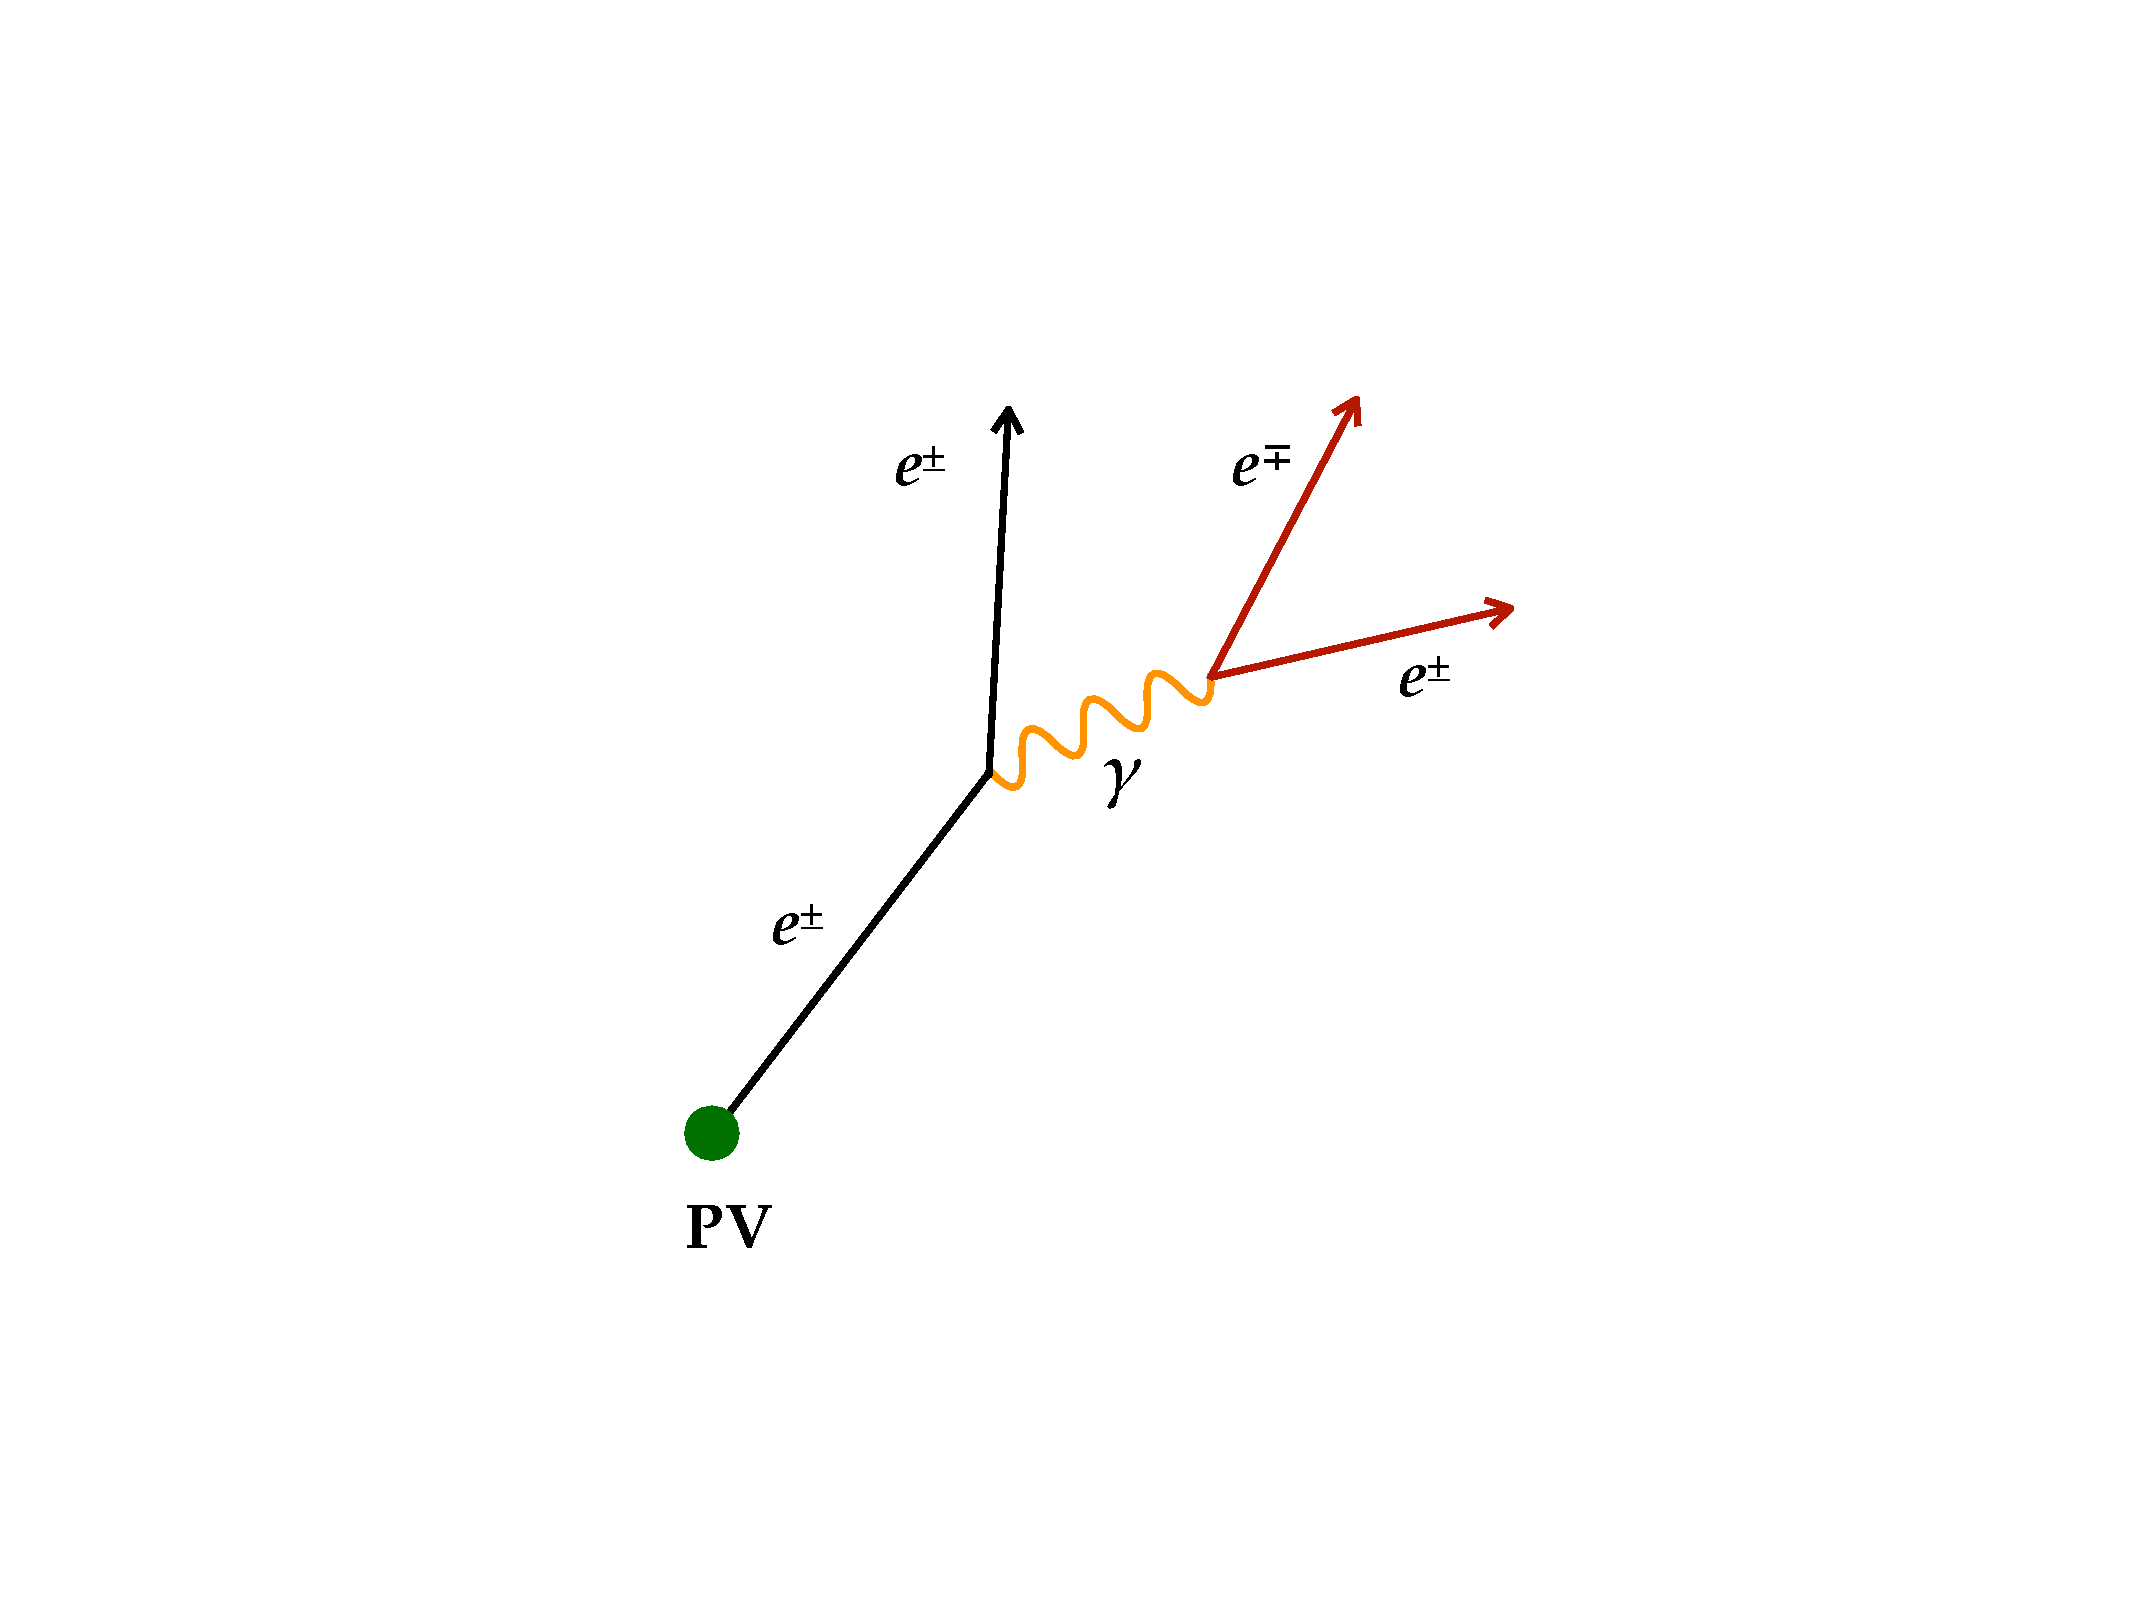
\includegraphics[width=0.45\textwidth]{figures/common_ana/fakes/electron_brem_fake}
        \caption{
        }
        \label{fig:electron_brem_fake}
    \end{center}
\end{figure}


%%%%%%%%%%%%%%%%%%%%%%%%%%%%%%%%%%%%%%%%%%%%%%%%%%%%%%%%%%%%%%%%%%%
%%%%%%%%%%%%%%%%%%%%%%%%%%%%%%%%%%%%%%%%%%%%%%%%%%%%%%%%%%%%%%%%%%%
%
% SOURCES OF FAKE MUONS
%
%%%%%%%%%%%%%%%%%%%%%%%%%%%%%%%%%%%%%%%%%%%%%%%%%%%%%%%%%%%%%%%%%%%
%%%%%%%%%%%%%%%%%%%%%%%%%%%%%%%%%%%%%%%%%%%%%%%%%%%%%%%%%%%%%%%%%%%
\subsubsection{Sources of Fake Muons}
\label{sec:fake_muon_sources}

As described in Section~\ref{sec:muons}, muons are primarily reconstructed via the combination
of tracking information provided by the ID and MS, and, generally speaking, they should be the only particle species to reach
the MS.
In addition to the semi-leptonic decays of heavy-flavored jets described above, however,
there are several sources of fake muons.
Highly energetic jets can have elongated shower profiles that reach the outer
radii of the hadronic calorimeter, with a non-zero chance of exiting the calorimeter
and resulting in particle leakage into the MS.
Such cases are referred to as calorimeter punch-through, and have been illustrated
in Figure~\ref{fig:jet_punch_through}.
Punch-through particles can leave signatures similar to charged muons whose subsequent
MS tracks are associated with a track in the ID, leading to a reconstructed combined muon
faking a genuine muon.
An additional source of fake muons come from the in-flight decays of charged hadrons,
such as the $K^\pm$ that can decay to $\mu^{\pm} \nu$.
Non-prompt muons arising as a result of such in-flight decays are typically
characterised by combined tracks that exhibit a kink topology, mentioned briefly
in the discussion of muon combined reconstruction in Section~\ref{sec:muon_id} and
illustrated in Figure~\ref{fig:fake_muon_kink}.

\begin{figure}[!htb]
    \begin{center}
        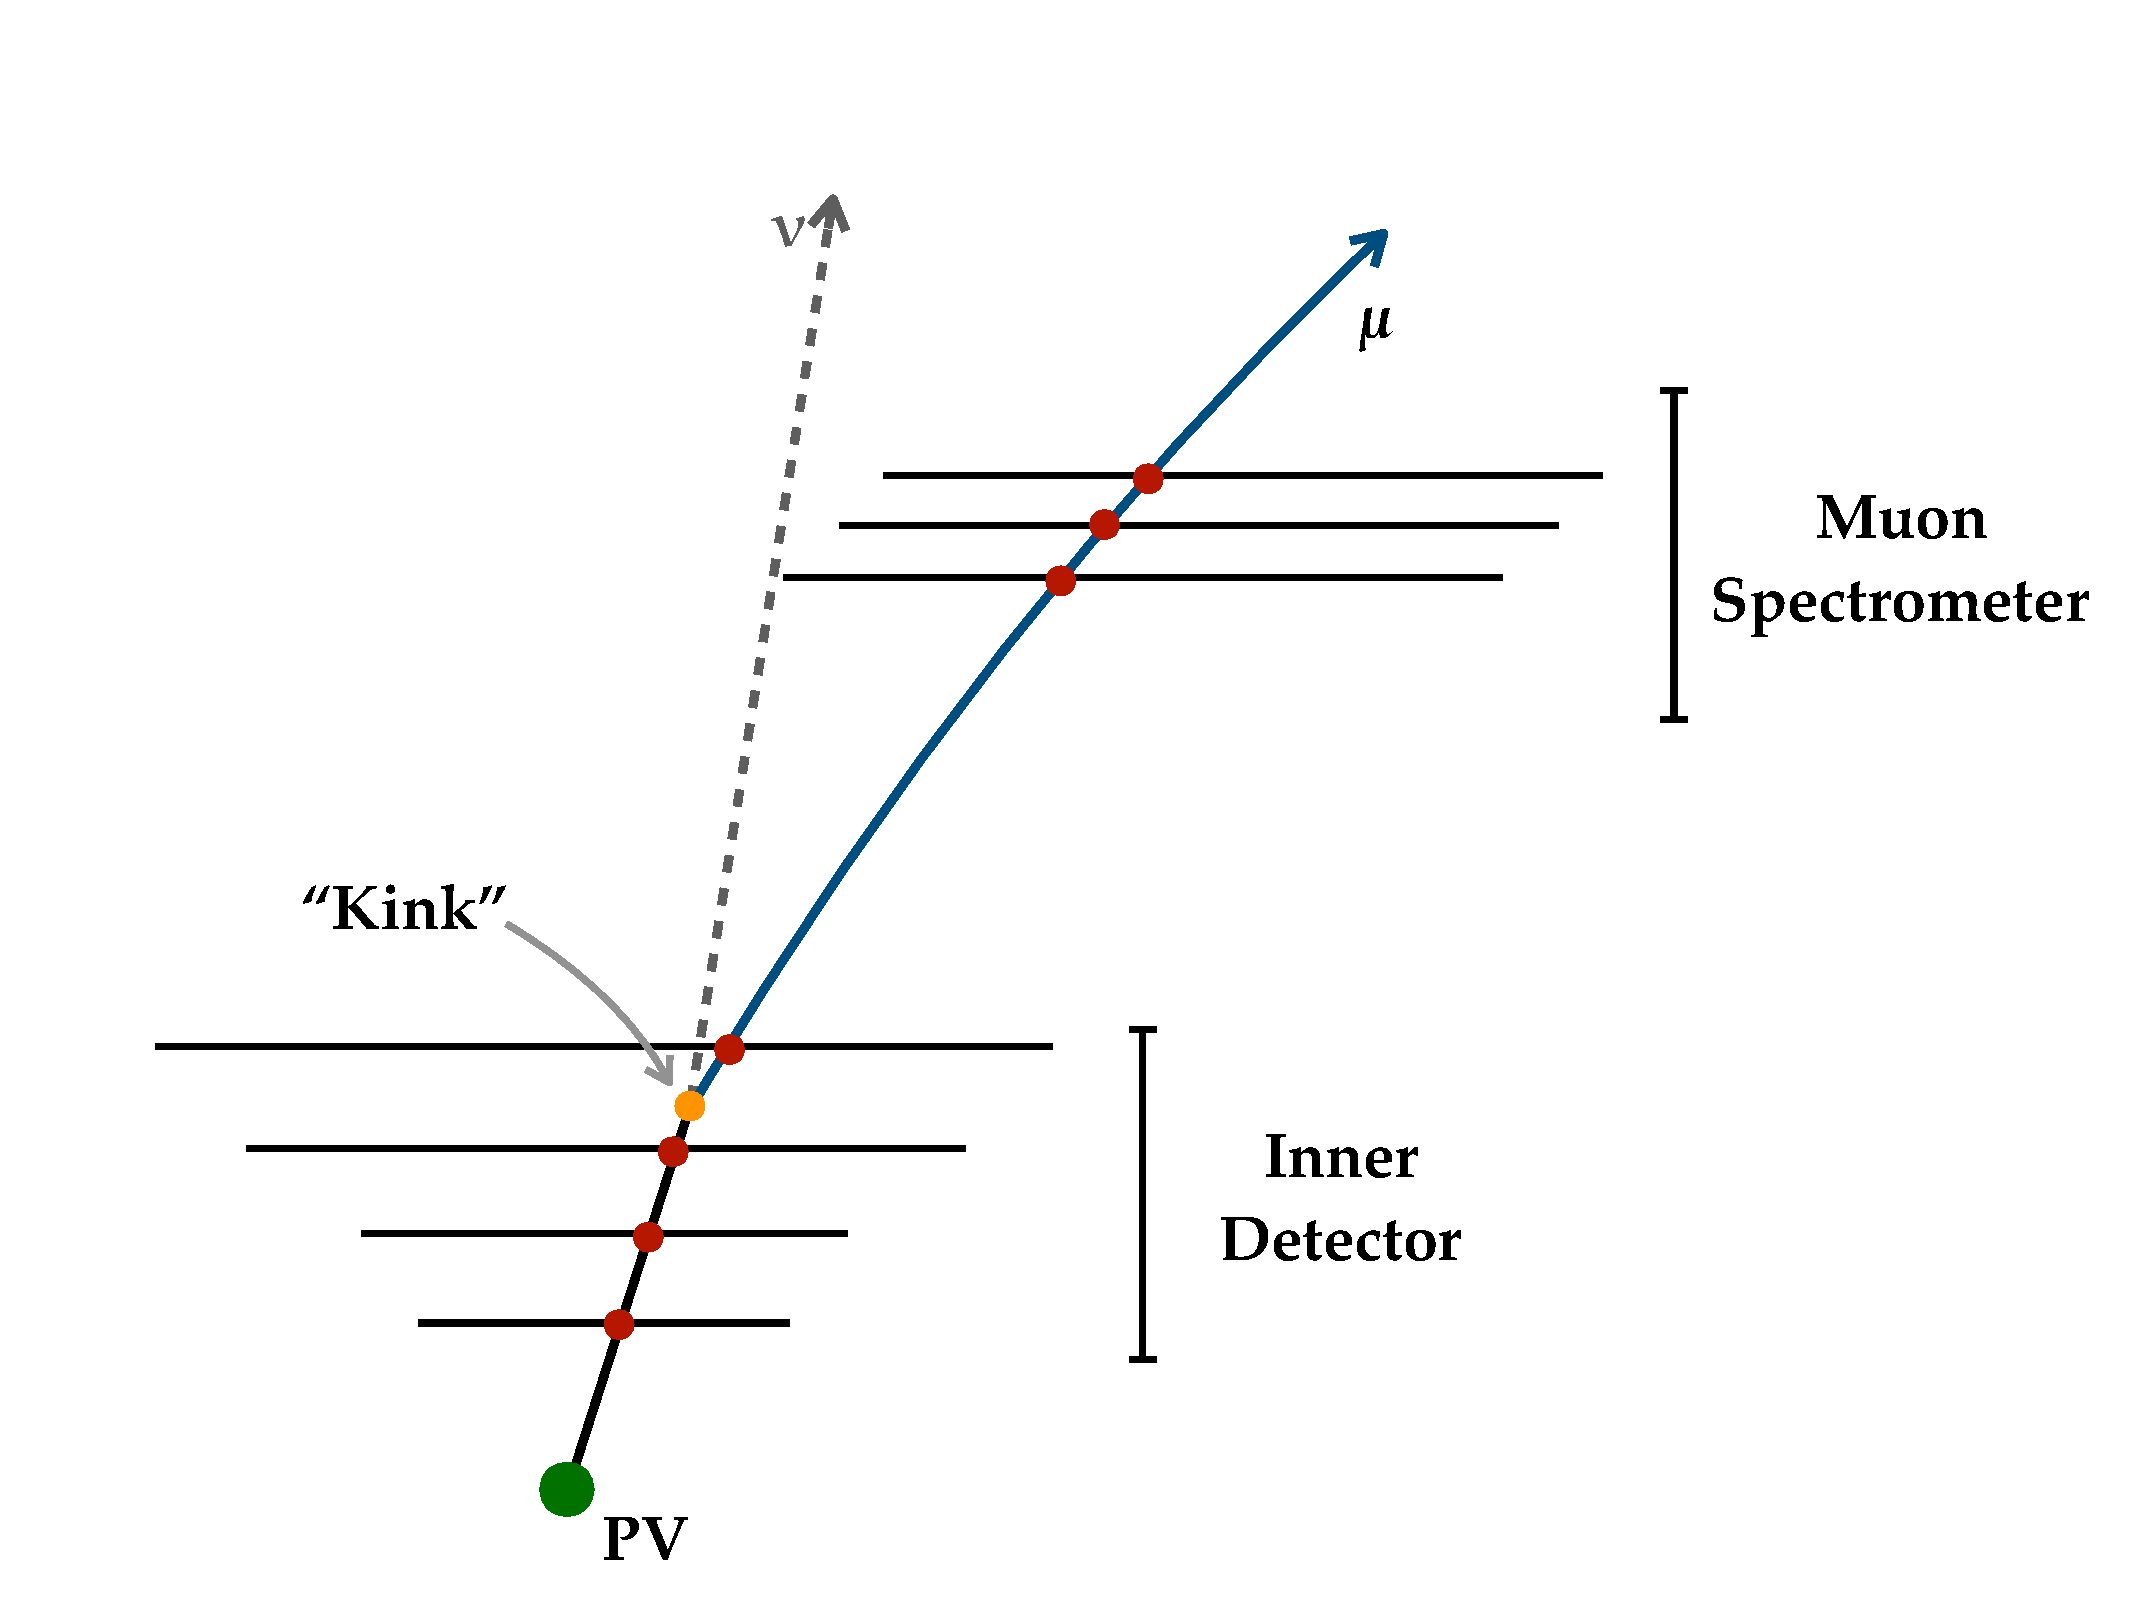
\includegraphics[width=0.65\textwidth]{figures/common_ana/fake_muon_kinkPDF}
        \caption{
            Illustration of a reconstructed non-prompt muon resulting from a kinked-track topology.
            A promptly produced hadron is produced and decays to a final state including a
            high-\pT muon.
            The point at which the hadron decays is indicated by the yellow dot.
            An example of such a decay is the decay $K^+ \rightarrow \mu^+ \nu$.
            The red circles indicate detector hits in the ID and MS layers indicated
            by the horizontal black lines.
            Implied particle lifetimes and detector sizes are not to scale.
        }
        \label{fig:fake_muon_kink}
    \end{center}
\end{figure}


%%%%%%%%%%%%%%%%%%%%%%%%%%%%%%%%%%%%%%%%%%%%%%%%%%%%%%%%%%%%%%%%%%%
%%%%%%%%%%%%%%%%%%%%%%%%%%%%%%%%%%%%%%%%%%%%%%%%%%%%%%%%%%%%%%%%%%%
%
% DATA DRIVEN MOTIVATION
%
%%%%%%%%%%%%%%%%%%%%%%%%%%%%%%%%%%%%%%%%%%%%%%%%%%%%%%%%%%%%%%%%%%%
%%%%%%%%%%%%%%%%%%%%%%%%%%%%%%%%%%%%%%%%%%%%%%%%%%%%%%%%%%%%%%%%%%%
\subsection{The Need for a Data-driven Approach}
\label{sec:fake_dd_motivation}

In the analyses to be presented in Chapters~\ref{chap:search_stop} and \ref{chap:search_hh},
relatively tight identification working points are used for electrons and muons.
As a result, the contamination of fake leptons in these analyses is relatively
minor.
Although small, their contamination does have measurable effects and so their contribution
must be accounted for in order to achieve accurate estimates of the backgrounds
in each analysis.

Several methods exist to estimate the background rates arising from the sources of fake
leptons, those relying on data-driven methods or those based entirely on the MC
simulation.
Relying on the MC simulation of these sources of fake leptons, described in previous
sections, means to rely entirely on the \textsc{GEANT4} simulation of the ATLAS detector
and on the MC generation and showering processes to accurately predict the
rates of these processes.
There are several problems with this approach and they are (nonexhaustively) as follows.
Given the very small region of phase space being probed by the analysis,
the number of MC events needed to appropriately sample the sources of production of fake
leptons as described above would be prohibitively large if a statistically relevant sample
is desired.
An accurate prediction of the production rates of several of these fake lepton sources
would require an accurate underlying theoretical model of many processes, such as
heavy-flavor jet fragmentation, which is challenging.
Additionally, many sources of fake leptons arise as a result of detector material interactions
or as a result of subtle and difficult-to-model failure modes of the detector response.
%or inaccurate simulation of the detector response.
The accurate prediction of the rate of photon conversions, for example, requires
high levels of precision in the simulation and measurement of the active and passive material in the ATLAS detector and cavern,
which is not necessarily possible.
The rates of jets being mis-identified as electrons and jet punch-through, for example,
require that the MC simulation of the calorimeter response and shower evolution are
accurately modelled.
The MC simulation is not expected to perform to the degree at which these subtle, and comparatively rare, effects
are accurately predicted.
For this reason, data-driven approaches are typically taken for estimating the background rates
of these fake lepton sources.
In the analyses to be presented, two data-driven approaches are taken.
In the search described in Chapter~\ref{chap:search_stop}, the Matrix Method
is used.
In the search described in Chapter~\ref{chap:search_hh}, the Same-sign Extrapolation
Method is used.
These methods are introduced in Sections~\ref{sec:matrix_method} and \ref{sec:same_sign_extrap}, respectively.


\FloatBarrier
%%%%%%%%%%%%%%%%%%%%%%%%%%%%%%%%%%%%%%%%%%%%%%%%%%%%%%%%%%%%%%%%%%%
%%%%%%%%%%%%%%%%%%%%%%%%%%%%%%%%%%%%%%%%%%%%%%%%%%%%%%%%%%%%%%%%%%%
%
% THE MATRIX METHOD
%
%%%%%%%%%%%%%%%%%%%%%%%%%%%%%%%%%%%%%%%%%%%%%%%%%%%%%%%%%%%%%%%%%%%
%%%%%%%%%%%%%%%%%%%%%%%%%%%%%%%%%%%%%%%%%%%%%%%%%%%%%%%%%%%%%%%%%%%
\subsection{The Matrix Method}
\label{sec:matrix_method}

The Matrix Method, discussed thoroughly in Ref.~\cite{TOPFake}, is one of the most common
methods used in ATLAS analyses for estimating backgrounds due to processes containing
fake leptons.
It is characterised by the definition of two levels of lepton selections:
\begin{itemize}
    \item[]\textbf{Tight Leptons}: Those leptons passing all reconstruction, identification, and isolation criteria
        as the leptons used in the final analysis' results
    \item[]\textbf{Loose Leptons}: Leptons requiring similar selections as the Tight leptons but typically with either, or both, identification
        and isolation criteria relaxed
\end{itemize}
The Tight leptons are a subset of the Loose, by definition.
In the analysis described in Chapter~\ref{chap:search_stop}, the Loose leptons are defined by loosening
only the lepton identification working points.
Generally speaking, both samples of Loose and Tight leptons will contain
both fake and real leptons.\footnote{Genuine, prompt
leptons originating from the $pp$ hard-scatter interaction point are typically referred to as `real' leptons
in order to distinguish them, semantically, from fake and non-prompt leptons.
}
The Matrix Method consists of measuring a set of efficiencies: the \textit{real}
(\textit{fake}) \textit{efficiencies}, $\varepsilon_r$ ($\varepsilon_f$),
defined as the efficiency for a real (fake) electron or muon that satisfies the Loose selection criteria
to also satisfy the Tight selection criteria.
This is illustrated in Figure~\ref{fig:fake_effs}.
As illustrated, both the Loose and Tight lepton samples will contain contributions of both fake
and real leptons.
The Matrix Method can be generalised to final states with any number of leptons.
In the discussion to follow, we will discuss that of final states with two leptons: the dilepton Matrix Method.

\begin{figure}[!htb]
    \begin{center}
        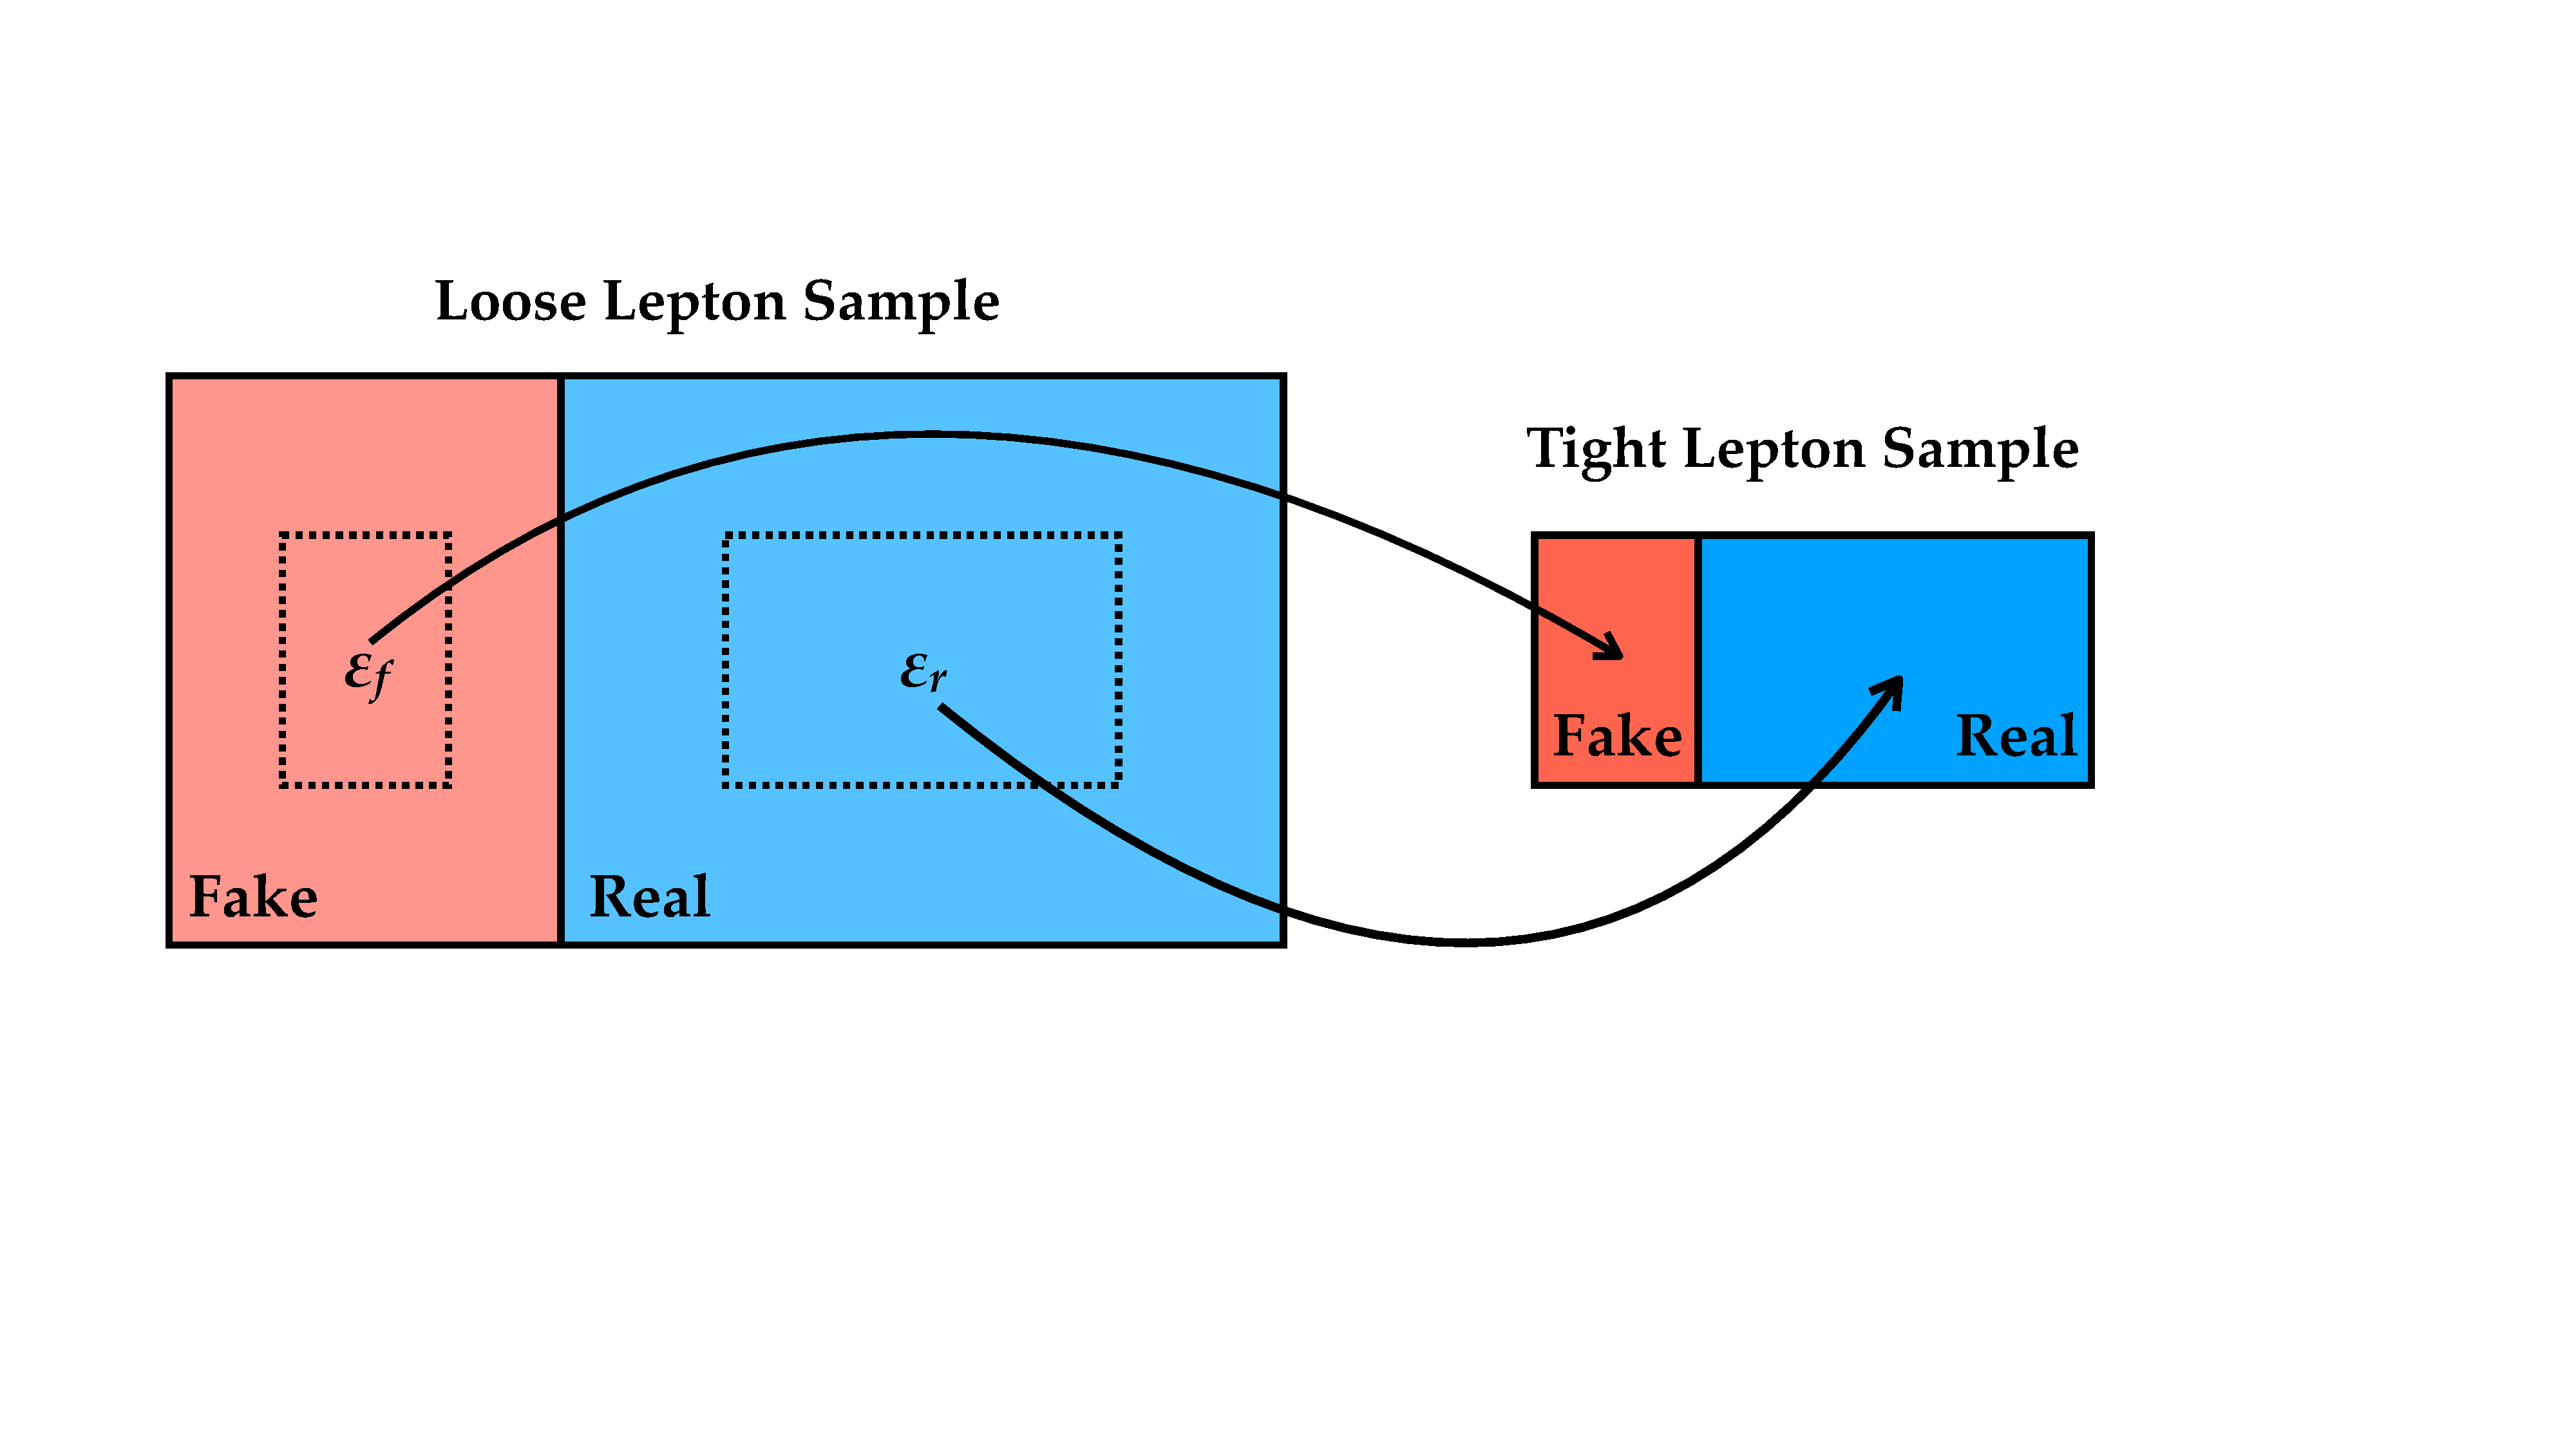
\includegraphics[width=0.65\textwidth]{figures/common_ana/fakes/fake_effs_illustration}
        \caption{
        }
        \label{fig:fake_effs}
    \end{center}
\end{figure}

The real efficiencies, $\varepsilon_r$, are measured in data using $Z$-boson tag-and-probe methods, requiring the probe lepton
to satisfy the Tight lepton selection and to be matched to the trigger.
The probe lepton must satisfy the Loose lepton selection.
The fraction of loose probe leptons to pass the Tight lepton selection then gives a measure of $\varepsilon_r$.

The fake efficiencies, $\varepsilon_f$, are measured in data using events with different-flavor leptons,
where one lepton is an electron and the other is a muon, that have the same electric charge.
A tag-and-probe method similar to that used in the measurement of $\varepsilon_r$ is used
and relies on the fact that a comparatively small amount of SM processes can result in same-sign
and different-flavor events.
Therefore, when a probe satisfies the Tight selection it is very likely to be the case that the
probe lepton is a fake lepton.
An additional component of the $\varepsilon_f$ is measured by additionally requesting that there
be at least one $b$-tagged jet in the same-sign, different-flavor selection.
This allows for $\varepsilon_f$ to be measured in a region enriched in fake leptons originating
from semi-leptonic decays of heavy-flavor jets.
The various measurements of $\varepsilon_f$ are combined following an averaging scheme, weighted according
to the composition of fake lepton sources expected to contaminate the SRs.

The real and fake efficiencies are not global quantities.
Instead, they are measured as a function of both the lepton $\pT$ and $\eta$
such that they may track the effects of changes in detector response and
material interaction over the $\pT$ and $\eta$ ranges relevant to the leptons used in the analysis.

Once $\varepsilon_r$ and $\varepsilon_f$ are obtained, the fake lepton background
can be obtained by inverting the equation relating the measured quantities (Tight versus Loose), taken
from the observed data, in terms
of those that we want to know (Fake versus Real):
\begin{equation}
    \begin{pmatrix}
        N_{TT} \\ N_{TL} \\ N_{LT} \\ N_{LL}
    \end{pmatrix}
        = M
    \begin{pmatrix}
        N_{LL}^{RR} \\ N_{LL}^{RF} \\ N_{LL}^{FR} \\ N_{LL}^{FF}
    \end{pmatrix}
    \label{eq:matrix_method}
\end{equation}
\noindent where in the sub- and super-scripts, the first (second) index refers to the leading (sub-leading) lepton.
The sub-script `$T$' (`$L$') refers to the lepton passing the Tight (Loose) lepton
selection.
The super-script `$R$' (`$F$') indicates whether or not the lepton is a real (fake) lepton.
For example, the quantity $N_{LL}^{FR}$ is the number of events in which the leading lepton
in the sample of Loose leptons is fake and the sub-leading is real.
The matrix $M$ is given by,
\begin{align}
    M = \begin{pmatrix}
            r_1 r_2 & r_1 f_2  & f_1 r_2 & f_1 f_2 \\
            r_1 \overline{r_2} & r_1\overline{f_2} & f_1 \overline{r_2} & f_1 \overline{f_2} \\
            \overline{r_1} r_2 & \overline{r_1} f_2 & \overline{f_1} r_2 & \overline{f_1} f_2 \\
            \overline{r_1} \overline{r_2} & \overline{r_1} \overline{f_2} & \overline{f_1} \overline{r_2} & \overline{f_1} \overline{f_2}
        \end{pmatrix}
    \label{eq:matrix_method_matrix}
\end{align}
where $r_i$ ($f_i$) is shorthand for the real (fake) efficiency, $\varepsilon_r$ ($\varepsilon_f$),
and the notation $\overline{x_i}$ indicates $(1 - x_i)$.
%To make clear the data-driven aspect of the method:
%both sets of qauntities --- those appearing on the left-hand-side of Equation~\ref{eq:matrix_method} and the $r_i$ and $f_i$ ---
%are measured using the observed data.

The number of events with double-fake and single-fake leptons satisfying the analysis' Tight selection
($N_{TT}^{FF}$ and $N_{TT}^{RF} + N_{TT}^{FR}$, respectively) can then be obtained from the
number of events with double-fake and single-fake leptons satisfying the Loose selection
($N_{LL}^{FF}$ and $N_{LL}^{RF} + N_{LL}^{FR}$, respectively) through inversion
of Equation~\ref{eq:matrix_method}  and
noting the following relations,
\begin{align}
    N_{TT}^{RR} &= r_1 r_2 \cdot N_{LL}^{RR}  \label{eq:matrix_method_sol0}\\
    N_{TT}^{RF} &= r_1 f_2 \cdot N_{LL}^{RF}  \label{eq:matrix_method_sol1}\\
    N_{TT}^{FR} &= f_1 r_2 \cdot N_{LL}^{FR}  \label{eq:matrix_method_sol2}\\
    N_{TT}^{FF} &= f_1 f_2 \cdot N_{LL}^{FF}. \label{eq:matrix_method_sol3}
\end{align}
The quantities appearing on the right-hand-side of Equations~\ref{eq:matrix_method_sol0}-\ref{eq:matrix_method_sol3}
depend entirely on the observed data.
The number of events in the analysis' Tight selection that have at least one fake lepton is then given by the sum
$N_{TT}^{RF} + N_{TT}^{FR} + N_{TT}^{FF}$.
This gives a total integrated yield for the fake background contribution in the analysis'
Tight selection; however, from Equations~\ref{eq:matrix_method_sol1}-\ref{eq:matrix_method_sol3}
a set of per-event weighting factors (`fake weights'), depending only on the $\varepsilon_r(\pT,\eta)$ and
$\varepsilon_f(\pT,\eta)$ efficiency factors for the two leptons, can be defined.
These fake weights allow for kinematic distributions of the fake lepton background
sources to be populated
by appropriately applying them to the data sample consisting of leptons satisfying the analysis' Loose selection.



%%%%%%%%%%%%%%%%%%%%%%%%%%%%%%%%%%%%%%%%%%%%%%%%%%%%%%%%%%%%%%%%%%%
%%%%%%%%%%%%%%%%%%%%%%%%%%%%%%%%%%%%%%%%%%%%%%%%%%%%%%%%%%%%%%%%%%%
%
% SAME SIGN EXTRAPOLATION
%
%%%%%%%%%%%%%%%%%%%%%%%%%%%%%%%%%%%%%%%%%%%%%%%%%%%%%%%%%%%%%%%%%%%
%%%%%%%%%%%%%%%%%%%%%%%%%%%%%%%%%%%%%%%%%%%%%%%%%%%%%%%%%%%%%%%%%%%
\subsection{Same-sign Extrapolation Method}
\label{sec:same_sign_extrap}



